\section*{第七章 空间向量及其应用}

1. B 提示: 空间任意两个非零向量 $a,b,a//b$ 包括向量 $a$ 和 $b$ 同向共线和反向共线两种情况,即当 $a//b$ 时,有 $\langle a,b\rangle  = 0$ 或 $\langle \vv{a},\vv{b}\rangle  = \pi$ ,不能得到 $\langle \vv{a},\vv{b}\rangle  = 0$ ,充分性不成立.

$\langle \vv{a},\vv{b}\rangle  = 0$ ,则 $\vv{a}$ 和 $\vv{b}$ 方向相同,有 $\vv{a}//\vv{b}$ ,必要性成立;

故 “ $\vv{a}//\vv{b}$ ” 是 “ $\langle \vv{a},\vv{b}\rangle  = 0$ ” 的必要不充分条件.

2. A 提示: 如图, $\vv{DA} - \dfrac{1}{2}\left( {\vv{DB} + \vv{DC}}\right)  = \vv{DA} - \dfrac{1}{2}\left( {2\vv{DE}}\right)  = \vv{DA} - \vv{DE} = \vv{EA} =  - \vv{AE}$ .

\begin{center}
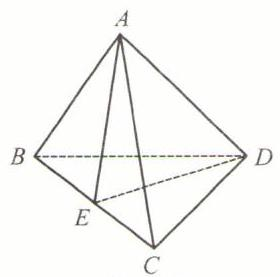
\includegraphics[width=0.2\textwidth]{bodyxb/src/bo_d20cdrf7aajc73bfmvhg_178_517_484_280_277_0.jpg}
\end{center}


(第 2 题)

\begin{center}
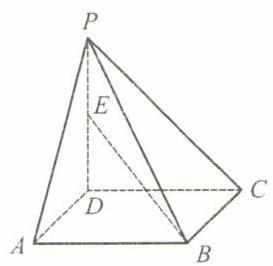
\includegraphics[width=0.2\textwidth]{bodyxb/src/bo_d20cdrf7aajc73bfmvhg_178_906_494_273_266_0.jpg}
\end{center}


(第 3 题)

3. $C$ 提示: 如图, $\vv{BE} = \vv{PE} - \vv{PB} = \dfrac{1}{2}\vv{PD} - \vv{PB} = \dfrac{1}{2}\left( {\vv{PB} + \vv{BD}}\right)  - \vv{PB} = \dfrac{1}{2}\left( {\vv{BD} - \vv{PB}}\right)$

$= \dfrac{1}{2}\left( {\vv{BA} + \vv{BC} - \vv{PB}}\right)  = \dfrac{1}{2}\left( {\vv{PA} - \vv{PB} + \vv{PC} - \vv{PB} - \vv{PB}}\right)$

$= \dfrac{1}{2}\vv{PA} - \dfrac{3}{2}\vv{PB} + \dfrac{1}{2}\vv{PC} = \dfrac{1}{2}a - \dfrac{3}{2}b + \dfrac{1}{2}c.$

4. $C$ 提示: $\vv{AB} = \vv{a} + 2\vv{b},\vv{BC} =  - 5\vv{a} + 6\vv{b},\vv{CD} = 7\vv{a} - 2\vv{b}$ .

对于选项 $A$ : 因为不存在任何 $\lambda  \in  \mathbf{R}$ ,使得 $\vv{BC} = \lambda \vv{AB}$ ,所以 $A,B,C$ 不共线,故 $A$ 错误.

对于选项 $B$ : 因为不存在任何 $\mu  \in  \mathbf{R}$ ,使得 $\vv{CD} = \mu \vv{BC}$ ,所以 $B,C,D$ 不共线,故 $B$ 错误.

对于选项 $C$ : 因为 $\vv{AD} = \vv{AB} + \vv{BC} + \vv{CD} = {3a} + {6b}$ ,所以 $\vv{AD} = 3\vv{AB}$ ,则 $A,B,D$ 三点共线,故 $C$ 正确.

对于选项 D: 因为 $\vv{AC} = \vv{AB} + \vv{BC} =  - {4a} + {8b}$ ,则不存在任何 $t \in  \mathbf{R}$ ,使得 $\vv{CD} = t\vv{AC}$ ,所以 $A,C,D$ 不共线,故 $D$ 错误.

5. B 提示:由 $\vv{OA} \cdot  \vv{OC} = \vv{OB} \cdot  \vv{OC}$ 得. $\vv{OC} \cdot  \left( {\vv{OB} - \vv{OA}}\right)  = \vv{OC} \cdot  \vv{AB} = 0$ ,所以 $\vv{OC}\bot \vv{AB}$ ,所以直线 ${AB}$ 与直线 ${OC}$ 的位置关系是垂直, 故选 B.

6. B 提示: 如图,因为 $M$ 为棱 ${AD}$ 的中点,

\begin{center}
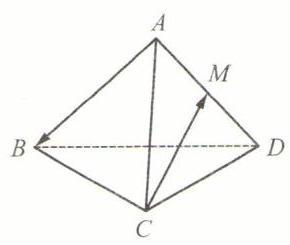
\includegraphics[width=0.2\textwidth]{bodyxb/src/bo_d20cdrf7aajc73bfmvhg_178_1236_1287_290_245_0.jpg}
\end{center}


(第 6 题)

所以 $\vv{AB} \cdot  \vv{CM} = \vv{AB} \cdot  \left( {\vv{CA} + \vv{AM}}\right)  = \vv{AB} \cdot  \left( {\vv{CA} + \dfrac{1}{2}\vv{AD}}\right)  =  - \vv{AB} \cdot  \vv{AC} + \dfrac{1}{2}\vv{AB} \cdot  \vv{AD}$ , 因为四面体 ${ABCD}$ 的棱长都是 2,所以 $\vv{AB} \cdot  \vv{CM} =  - 2 \times  2 \times  \dfrac{1}{2} + \dfrac{1}{2} \times  2 \times  2 \times  \dfrac{1}{2} =  - 2 + 1 =$ -1.

7. $A$ 提示:由正四棱柱性质可知,向量 $\vv{AP}$ 在 $\vv{A{A}_{1}}$ 上的投影向量为 $\vv{A{A}_{1}}$ ,由数量积的几何意义可知, $\vv{A{A}_{1}} \cdot  \vv{AP} = {\left| \vv{A{A}_{1}}\right| }^{2} = 1$ .

8. C 提示: $\vv{C{A}_{1}} \cdot  \left( {\vv{CB} + \vv{CA}}\right)  = \left( {\vv{C{C}_{1}} + \vv{CA}}\right)  \cdot  \left( {\vv{CB} + \vv{CA}}\right)  = \vv{C{C}_{1}} \cdot  \vv{CB} + \vv{C{C}_{1}} \cdot  \vv{CA} + \vv{CA} \cdot  \vv{CB} + \vv{C{A}^{2}} = 4 \times  4 \times  \cos \dfrac{\pi }{3} + 4$  $\times  4 \times  \cos \dfrac{\pi }{3} + 4 \times  4 \times  \cos \dfrac{\pi }{4} + {4}^{2} = 8 + 8 + 8\sqrt{2} + {16} = {32} + 8\sqrt{2}.$

9. $\sqrt{5}$ 提示:依题意, $a \cdot  b = b \cdot  c = c \cdot  a = \dfrac{1}{2}$ ,则 ${\left| a - b + 2c\right| }^{2} = {\left( a - b + 2c\right) }^{2} = {\left| a\right| }^{2} + {\left| b\right| }^{2} + 4{\left| c\right| }^{2} - {2a} \cdot  b - {4b} \cdot  c + {4a}$  $c = 6 - 2 \times  \dfrac{1}{2} - 4 \times  \dfrac{1}{2} + 4 \times  \dfrac{1}{2} = 5,\left| {a - b + {2c}}\right|  = \sqrt{5}.$

10. $\dfrac{1}{8}$ 提示: 由题意得 ${\left| \vv{a} - \vv{b}\right| }^{2} = 7$ ,即 ${\vv{a}}^{2} - 2\vv{a} \cdot  \vv{b} + {\vv{b}}^{2} = 7$ ,则 $\vv{a} \cdot  \vv{b} = \dfrac{1}{2}$ ,则 $\cos \langle \vv{a},\vv{b}\rangle  = \dfrac{\vv{a} \cdot  \vv{b}}{\left| \vv{a}\right| \left| \vv{b}\right| } = \dfrac{\dfrac{1}{2}}{2 \times  2} = \dfrac{1}{8}$ .

11. $\dfrac{1}{2}a - \dfrac{1}{4}b + \dfrac{1}{2}c$ 提示: $\because E$ 为 ${AC}$ 中点, $\therefore \vv{PE} = \dfrac{1}{2}\left( {\vv{PA} + \vv{PC}}\right)$ . $\because \vv{BF} = 3\vv{FP},\therefore \vv{PF} = \dfrac{1}{4}\vv{PB}$ .

$\therefore \vv{FE} = \vv{PE} - \vv{PF} = \dfrac{1}{2}\left( {\vv{PA} + \vv{PC}}\right)  - \dfrac{1}{4}\vv{PB} = \dfrac{1}{2}a - \dfrac{1}{4}b + \dfrac{1}{2}c$ .

12. $\dfrac{1}{6}$ 提示:因为 $\vv{MA},\vv{MB},\vv{MC}$ 共面,所以 $M,A,B,C$ 四点共面,又 $\vv{OM} = \dfrac{1}{2}\vv{OA} + \dfrac{1}{3}\vv{OB} + \lambda \vv{OC}$ ,根据四点共面的充要条件可得 $\dfrac{1}{2} + \dfrac{1}{3} + \lambda  = 1$ ,解得 $\lambda  = \dfrac{1}{6}$ .

13. $\dfrac{5}{3}$ 提示: 空间向量 $\vv{PA},\vv{PB},\vv{PC}$ 的模长分别为1,2,3,且两两夹角均为 $\dfrac{\pi }{3}$ ,如图,

\begin{center}
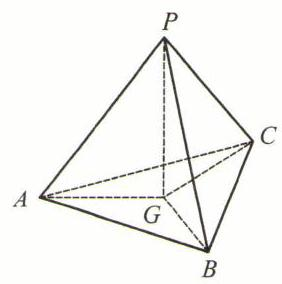
\includegraphics[width=0.2\textwidth]{bodyxb/src/bo_d20cdrf7aajc73bfmvhg_179_1132_260_282_284_0.jpg}
\end{center}


(第 13 题)

由 $G$ 为 $\bigtriangleup {ABC}$ 的重心,得 $\vv{GA} + \vv{GB} + \vv{GC} = \mathbf{0}$ .

于是 $\vv{PA} - \vv{PG} + \vv{PB} - \vv{PG} + \vv{PC} - \vv{PG} = \mathbf{0}$ ,即 $3\vv{PG} = \vv{PA} + \vv{PB} + \vv{PC}$ ,

所以 $\left| \vv{PG}\right|  = \dfrac{1}{3}\sqrt{{\left( \vv{PA} + \vv{PB} + \vv{PC}\right) }^{2}} =$

$\dfrac{1}{3}\sqrt{\vv{PA}{}^{2} + \vv{PB}{}^{2} + \vv{PC}{}^{2} + 2\left( {\vv{PA} \cdot  \vv{PB} + \vv{PB} \cdot  \vv{PC} + \vv{PC} \cdot  \vv{PA}}\right) }$

$= \dfrac{1}{3}\sqrt{1 + 4 + 9 + 2 \times  \left( {1 \times  2\cos \dfrac{\pi }{3} + 2 \times  3\cos \dfrac{\pi }{3} + 1 \times  3\cos \dfrac{\pi }{3}}\right) } = \dfrac{5}{3}.$

14. $\dfrac{\sqrt{10}}{2}$ 提示: 设 $\vv{AO} = \vv{a},\vv{AB} = \vv{b},\vv{AC} = \mathbf{c}$ ,

$\vv{DE} = \vv{DA} + \vv{AB} + \vv{BE} = \dfrac{1}{2}\vv{OA} + \vv{AB} + \dfrac{1}{2}\left( {\vv{AC} - \vv{AB}}\right)  =  - \dfrac{1}{2}\vv{AO} + \dfrac{1}{2}\vv{AB} + \dfrac{1}{2}\vv{AC} =  - \dfrac{1}{2}\vv{a} + \dfrac{1}{2}\vv{b} + \dfrac{1}{2}\mathbf{c},$

$\left| \vv{DE}\right|  = \sqrt{{\left( -\dfrac{1}{2}a + \dfrac{1}{2}b + \dfrac{1}{2}c\right) }^{2}} = \dfrac{1}{2}\sqrt{{\left( -a + b + c\right) }^{2}} = \dfrac{1}{2}\sqrt{{a}^{2} + {b}^{2} + {c}^{2} - {2a} \cdot  b - {2a} \cdot  c + {2b} \cdot  c}$

$= \dfrac{1}{2}\sqrt{1 + 1 + 9 - 2 \times  1 \times  1 \times  \cos {60}^{ \circ  } - 2 \times  1 \times  3 \times  \cos {60}^{ \circ  } + 2 \times  1 \times  3 \times  \cos {60}^{ \circ  }} = \dfrac{1}{2}\sqrt{{11} - 1 - 3 + 3} = \dfrac{\sqrt{10}}{2}$ ,故 ${DE} = \dfrac{\sqrt{10}}{2}$ .

15. (1) 8 个,分别为 $\vv{A{A}_{1}},\vv{{A}_{1}A},\vv{B{B}_{1}},\vv{{B}_{1}B},\vv{C{C}_{1}},\vv{{C}_{1}C},\vv{D{D}_{1}},\vv{{D}_{1}D}$ .

(2) $\vv{{A}_{1}{B}_{1}},\vv{DC},\vv{{D}_{1}{C}_{1}}$ .

(3) $\vv{{A}_{1}A},\vv{{B}_{1}B},\vv{{C}_{1}C},\vv{{D}_{1}D}$ .

16. 因为 $\vv{MN} = \vv{PN} - \vv{PM} = \dfrac{1}{2}\vv{PD} - \dfrac{2}{3}\vv{PC} = \dfrac{1}{2}\vv{AD} - \dfrac{1}{2}\vv{AP} - \dfrac{2}{3}\vv{AC} + \dfrac{2}{3}\vv{AP} = \dfrac{1}{2}\vv{AD} - \dfrac{2}{3}\vv{AB} - \dfrac{2}{3}\vv{BC} + \dfrac{1}{6}\vv{AP} =  - \dfrac{2}{3}\vv{AB}$  $- \dfrac{1}{6}\vv{AD} + \dfrac{1}{6}\vv{AP}$ ,所以, $x =  - \dfrac{2}{3},y =  - \dfrac{1}{6},z = \dfrac{1}{6}$ .

17. $\vv{AM} = \vv{AB} + \vv{BM} = \vv{AB} + \dfrac{1}{2}\left( {\vv{BC} + \vv{BB}}\right)  = \vv{AB} + \dfrac{1}{2}\vv{BB} + \dfrac{1}{2}\left( {\vv{AC} - \vv{AB}}\right)  = \vv{AB} + \dfrac{1}{2}\vv{A{A}^{\prime }} + \dfrac{1}{2}\left( {\vv{AC} - \vv{AB}}\right)  = \vv{b} + \dfrac{1}{2}\vv{a} +$  $\dfrac{1}{2}\left( {\mathbf{c} - \vv{b}}\right)  = \vv{b} + \dfrac{1}{2}\vv{a} + \dfrac{1}{2}\mathbf{c} - \dfrac{1}{2}\vv{b} = \dfrac{1}{2}\vv{a} + \dfrac{1}{2}\vv{b} + \dfrac{1}{2}\mathbf{c}$ ,即 $\vv{AM} = \dfrac{1}{2}\vv{a} + \dfrac{1}{2}\vv{b} + \dfrac{1}{2}\mathbf{c}.$  $\vv{AN} = \vv{A{A}^{\prime }} + \vv{{A}^{\prime }N} = \vv{A{A}^{\prime }} + \dfrac{1}{2}\left( {\vv{{A}^{\prime }{B}^{\prime }} + \vv{{A}^{\prime }{C}^{\prime }}}\right)  = \vv{A{A}^{\prime }} + \dfrac{1}{2}\vv{AB} + \dfrac{1}{2}\vv{AC} = \vv{a} + \dfrac{1}{2}\vv{b} + \dfrac{1}{2}\mathbf{c}$ 18. 因为 $\vv{AB} = 4\vv{a} + 5\vv{b} + 3\mathbf{c},\vv{AC} = 2\vv{a} + 3\vv{b} + \mathbf{c},\vv{AD} = 6\vv{a} + 7\vv{b} + 5\mathbf{c}$ , 所以 $\vv{BC} = \vv{AC} - \vv{AB} = {2a} + {3b} + c - \left( {{4a} + {5b} + {3c}}\right)  =  - {2a} - {2b} - {2c}$ , $\vv{BD} = \vv{AD} - \vv{AB} = {6\vv{a}} + {7\vv{b}} + {5\mathbf{c}} - \left( {{4\vv{a}} + {5\vv{b}} + {3\mathbf{c}}}\right)  = {2\vv{a}} + {2\vv{b}} + {2\mathbf{c}}$ . 所以 $\vv{BC} =  - \vv{BD}$ ,所以 $\vv{BC}//\vv{BD}$ ,又 $B$ 为公共点,所以 $B,C,D$ 三点共线. 19. (1)在正四面体 ${ABCD}$ 中, $E,F$ 分别为棱 ${BC},{CD}$ 的中点,点 $G$ 为线段 ${AF}$ 的中点,

\[
\vv{AG} = \dfrac{1}{2}\vv{AF} = \dfrac{1}{2} \times  \dfrac{1}{2}\left( {\vv{AC} + \vv{AD}}\right)  = \dfrac{1}{4}\vv{AC} + \dfrac{1}{4}\vv{AD},
\]

$\vv{AE} = \dfrac{1}{2}\left( {\vv{AB} + \vv{AC}}\right)$ ,所以 $\vv{EG} = \vv{AG} - \vv{AE} = \dfrac{1}{4}\vv{AC} + \dfrac{1}{4}\vv{AD} - \dfrac{1}{2}\vv{AB} - \dfrac{1}{2}\vv{AC} =  - \dfrac{1}{2}\vv{AB} - \dfrac{1}{4}\vv{AC} + \dfrac{1}{4}\vv{AD}$ . ( 2 )正四面体 ${ABCD}$ 的棱长为 1,则 $\vv{AB} \cdot  \vv{AC} = \vv{AB} \cdot  \vv{AD} = 1 \times  1 \times  \cos {60}^{ \circ  } = \dfrac{1}{2}$ , 所以 $\vv{EG} \cdot  \vv{AB} =  - \dfrac{1}{4}\left( {2\vv{AB} + \vv{AC} - \vv{AD}}\right)  \cdot  \vv{AB} =  - \dfrac{1}{4}\left( {2{\vv{AB}}^{2} + \vv{AC} \cdot  \vv{AB} - \vv{AD} \cdot  \vv{AB}}\right)  =  - \dfrac{1}{2}$ . 20. (1) ${\vv{CA}}_{1}^{2} = {\left( \vv{CD} + \vv{CB} + \vv{C{C}_{1}}\right) }^{2} = {\vv{CD}}^{2} + {\vv{CB}}^{2} + {\vv{CC}}_{1}^{2} + 2\left( {\vv{CD} \cdot  \vv{CB} + \vv{CD} \cdot  \vv{C{C}_{1}} + \vv{CB} \cdot  \vv{C{C}_{1}}}\right)  = 1 + 1 + 4 +$  $2\left( {1 \times  1 \times  \cos {60}^{ \circ  } + 1 \times  2 \times  \cos {60}^{ \circ  } + 1 \times  2 \times  \cos {60}^{ \circ  }}\right)  = {11}$ ,所以 ${A}_{1}C$ 的长为 $\sqrt{11}$ .

(2) $\vv{C{A}_{1}} \cdot  \vv{D{C}_{1}} = \left( {\vv{CD} + \vv{CB} + \vv{C{C}_{1}}}\right)  \cdot  \left( {\vv{C{C}_{1}} - \vv{CD}}\right)  = \vv{CD} \cdot  \vv{C{C}_{1}} - \vv{CD} \cdot  \vv{CD} + \vv{CB} \cdot  \vv{C{C}_{1}} - \vv{CB} \cdot  \vv{CD} + \vv{C{C}_{1}} \cdot  \vv{C{C}_{1}} -$  $\vv{C{C}_{1}} \cdot  \vv{CD} = 1 - 1 + 1 - \dfrac{1}{2} + 4 - 1 = \dfrac{7}{2}$ . 易求得 $\left| \vv{D{C}_{1}}\right|  = \sqrt{3}$ .

设异面直线 $C{A}_{1}$ 与 $D{C}_{1}$ 所成角为 $\theta$ ,故 $\cos \theta  = \left| {\cos \left\langle  {\vv{C{A}_{1}},\vv{D{C}_{1}}}\right\rangle  }\right|  = \dfrac{\left| \vv{C{A}_{1}} \cdot  \vv{D{C}_{1}}\right| }{\left| \vv{C{A}_{1}}\right|  \cdot  \left| \vv{D{C}_{1}}\right| } = \dfrac{7\sqrt{33}}{66}$ ,所以 $C{A}_{1}$ 与 $D{E}_{1}$ 所成角的余弦值为 $\dfrac{7\sqrt{33}}{66}$ .

21. B 提示: 当 $\langle \vv{a},\vv{b}\rangle  = \pi$ 时,满足 $\vv{a} \cdot  \vv{b} < 0$ ,但 $\langle \vv{a},\vv{b}\rangle$ 不是钝角,故 A 错误.

\begin{center}
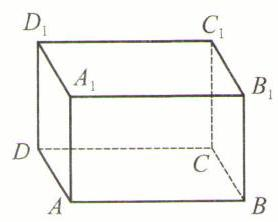
\includegraphics[width=0.2\textwidth]{bodyxb/src/bo_d20cdrf7aajc73bfmvhg_180_1199_192_278_222_0.jpg}
\end{center}


(第 21 题)

当 $\vv{AB} + \vv{CD} = \mathbf{0}$ 时, $\vv{AB} =  - \vv{CD}$ ,所以 $\vv{AB}$ 与 $\vv{CD}$ 一定共线,故 $B$ 正确.

当 $\vv{AB} = \vv{CD}$ 时,则 $\vv{AB}$ 与 $\vv{CD}$ 共线,但线段 ${AB}$ 与 ${CD}$ 可能只是平行关系,故 $C$ 错误.

如图所示:

设 $\vv{AB} = \vv{a},\vv{AD} = \vv{b},\vv{A{A}_{1}} = \mathbf{c}$ ,显然满足 $\vv{a}$ 与 $\vv{b},\vv{b}$ 与 $\mathbf{c},\mathbf{c}$ 与 $\vv{a}$ 都是共面向量,但 $\vv{a},\vv{b},\mathbf{c}$ 不共面, 故 D 错误.

22. $C$ 提示: 对于选项 $A$ ,由于两条不同直线 $l,m$ 的方向向量为 ${v}_{1},{v}_{2}$ ,当 $l//m$ 时, ${v}_{1}//{v}_{2}$ ,当 ${v}_{1}//$  ${v}_{2}$ 时, $l//m$ ,所以 $A$ 正确.

对于选项 $B$ ,因为 $\vv{OD} = \dfrac{1}{3}\vv{OA} + \dfrac{1}{3}\vv{OB} + \dfrac{1}{3}\vv{OC}$ ,所以 $3\vv{OD} - \vv{OA} - \vv{OB} - \vv{OC} = \mathbf{0}$ ,所以 $\left( {\vv{OD} - \vv{OA}}\right)  + \left( {\vv{OD} - \vv{OB}}\right)  +$  $\left( {\vv{OD} - \vv{OC}}\right)  = \mathbf{0}$ ,所以 $\vv{AD} + \vv{BD} + \vv{CD} = \mathbf{0}$ ,所以 $\vv{AD} = \vv{DB} + \vv{DC}$ .

设 $E$ 为 ${BC}$ 的中点,所以 $\vv{AD} = \vv{DB} + \vv{DC} = 2\vv{DE}$ ,所以 $\vv{AD} = \dfrac{2}{3}\vv{AE}$ ,所以 $D$ 在平面 ${ABC}$ 内,且 $D$ 为 $\bigtriangleup  {ABC}$ 的重心,所以 B 正确.

对于选项 $C$ ,因为 $a + b + c = \left( {a + b}\right)  + \dfrac{1}{2} \times  {2c}$ ,所以 $a + b,{2c},a + b + c$ 共面,所以 $\{ a + b,{2c},a + b + c\}$ 不是空间向量的一组基底,所以 $C$ 错误.

对于选项 $D$ ,由空间向量共面定理可知空间向量 $a,b,c$ 共面,则存在不全为 0 的实数 $x,y,z$ 使 ${xa} + {yb} + {zc} = 0$ ,所以 $D$ 正确.

23. $B$ 提示:若 $x + y + z = 1$ ,则 $\vv{OP} = \left( {1 - y - z}\right) \vv{OA} + y\vv{OB} + z\vv{OC}$ ,即 $\vv{AP} = y\vv{AB} + z\vv{AC}$ .

由共面定理可知向量 $\vv{AP},\vv{AB},\vv{AC}$ 共面,所以 $P,A,B,C$ 四点共面.

反之,若 $P,A,B,C$ 四点共面,当 $O$ 与四个点中的一个 (比如 $A$ 点) 重合时,

$\vv{OA} = \mathbf{0}$ , $x$ 可取任意值,不一定有 $x + y + z = 1$ ,所以 $x + y + z = 1$ 是 $P,A,B,C$ 四点共面的充分不必要条件.

24. $B$ 提示: 取 ${AB}$ 中点 $E$ ,可知 $E$ 在球面上,可得 $\vv{EB} =  - \vv{EA} =  - \dfrac{1}{2}\vv{BA}$ ,

\begin{center}
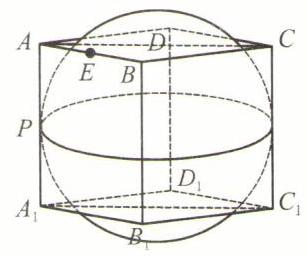
\includegraphics[width=0.2\textwidth]{bodyxb/src/bo_d20cdrf7aajc73bfmvhg_180_1177_1079_307_256_0.jpg}
\end{center}


(第 24 题)

所以 $\vv{PA} \cdot  \vv{PB} = \left( {\vv{PE} + \vv{EA}}\right)  \cdot  \left( {\vv{PE} + \vv{EB}}\right)  = {\left( \vv{PE}\right) }^{2} - {\left( \vv{EA}\right) }^{2} = {\vv{PE}}^{2} - \dfrac{1}{4}$ .

点 $P$ 在球面上运动,当 ${PE}$ 为直径时, ${\left| \vv{PE}\right| }_{\max } = \sqrt{2}$ ,

所以 $\vv{PA} \cdot  \vv{PB}$ 的最大值为 $\dfrac{7}{4}$ .

25. $C$ 提示:由已知得 ${\left| a\right| }^{2} \geq  4{\left| a + tb\right| }^{2}$ ,所以 $3{\left| a\right| }^{2} + {8ta} \cdot  b + 4{t}^{2}{\left| b\right| }^{2} \leq  0$ . 即存在实数 $t$ , 使得不等式 $4{t}^{2} + {16t} + 3{\left| a\right| }^{2} \leq  0$ 有解,则有 $\Delta  = {16}^{2} - 4 \times  4 \times  \left( {3{\left| a\right| }^{2}}\right)  \geq  0$ ,解得 $\left| \vv{a}\right|  \leq  \dfrac{4\sqrt{3}}{3},$

又因为 $\vv{a} \cdot  \vv{b} = 2$ 且 $\left| \vv{b}\right|  = 1$ ,所以 $\vv{a}$ 在 $\vv{b}$ 方向上的数量投影是 $\dfrac{\vv{a} \cdot  \vv{b}}{\left| \vv{b}\right| } = \dfrac{2}{1} = 2$ .

所以 $a$ 围成的空间几何体,高为 2,母线长为 $\dfrac{4\sqrt{3}}{3}$ 的圆锥,

则其底面半径为 $r = \sqrt{{\left( \dfrac{4\sqrt{3}}{3}\right) }^{2} - {2}^{2}} = \dfrac{2\sqrt{3}}{3}$ ,

故由 $a$ 构成的空间几何体的侧面积为 $\pi  \cdot  \dfrac{2\sqrt{3}}{3} \cdot  \dfrac{4\sqrt{3}}{3} = \dfrac{8\pi }{3}$ .

26. 4 提示: 由题意可得 $\vv{GP} + \left( {\vv{GP} + \vv{PA}}\right)  + \left( {\vv{GP} + \vv{PB}}\right)  + \left( {\vv{GP} + \vv{PC}}\right)  = \mathbf{0}$ ,

即可得 $4\vv{GP} + \vv{PA} + \vv{PB} + \vv{PC} = \mathbf{0}$ ,所以 $4\vv{PG} = \vv{PA} + \vv{PB} + \vv{PC}$ .

又 $\vv{PD} = x\vv{PA},\vv{PE} = y\vv{PB},\vv{PF} = z\vv{PC}$ ,所以 $\vv{PA} = \dfrac{1}{x}\vv{PD},\vv{PB} = \dfrac{1}{y}\vv{PE},\vv{PC} = \dfrac{1}{z}\vv{PF}$ ,

即 $4\vv{PG} = \vv{PA} + \vv{PB} + \vv{PC} = \dfrac{1}{x}\vv{PD} + \dfrac{1}{y}\vv{PE} + \dfrac{1}{z}\vv{PF}$ .

又 $G,D,E,F$ 四点共面,由空间向量共面定理可得 $\dfrac{1}{x} + \dfrac{1}{y} + \dfrac{1}{z} = 4$ .

27. $2\sqrt{17}$ 提示: 由题意得 $\vv{AC} \cdot  \vv{AB} = 0,\vv{BD} \cdot  \vv{AB} = 0$ ,

所以 $\vv{CD} = \vv{CA} + \vv{AB} + \vv{BD},{\vv{CD}}^{2} = {\left( \vv{CA} + \vv{AB} + \vv{BD}\right) }^{2} = {\vv{CA}}^{2} + {\vv{AB}}^{2} + {\vv{BD}}^{2} + 2\vv{CA} \cdot  \vv{BD} = {36} + {16} + {64} + 2 \times  6 \times  8 \times$  $\cos {120}^{ \circ  } = {68}$ ,所以 ${CD}$ 的长 $\left| \vv{CD}\right|  = \sqrt{68} = 2\sqrt{17}$ .

28. $\sqrt{2}$ 或 $\sqrt{6}$ 提示:由题意知, $\vv{FE} = \vv{FA} + \vv{A{A}_{1}} + \vv{{A}_{1}E}$ ,所以 ${\vv{FE}}^{2} = {\left( \vv{FA} + \vv{A{A}_{1}} + \vv{{A}_{1}E}\right) }^{2}$ ,

展开得 $\vv{F{E}^{2}} = \vv{F{A}^{2}} + \vv{A{A}_{1}}{}^{2} + \vv{{A}_{1}{E}^{2}} + 2\vv{FA} \cdot  \vv{A{A}_{1}} + 2\vv{FA} \cdot  \vv{{A}_{1}E} + 2\vv{A{A}_{1}} \cdot  \vv{{A}_{1}E}$ .

因为异面直线 $a,b$ 所成角为 ${60}^{ \circ  }$ ,所以向量 $\vv{AF},\vv{{A}_{1}E}$ 的夹角为 ${60}^{ \circ  }$ 或 ${120}^{ \circ  }$ .

因为 ${A}_{1}A \bot  a,{A}_{1}A \bot  b$ ,所以 $\vv{FA} \bot  \vv{A{A}_{1}},\vv{A{A}_{1}} \bot  \vv{{A}_{1}E}$ ,即 $\vv{FA} \cdot  \vv{A{A}_{1}} = \vv{A{A}_{1}} \cdot  \vv{{A}_{1}E} = 0$ .

且 ${A}_{1}E = 1,{AF} = 2,{EF} = 3$ ,代入可得 $9 = 4 + {\vv{A{A}_{1}}}^{2} + 1 + 0 \pm  2 \times  1 \times  2 \times  \cos {60}^{ \circ  } + 0$ ,

得方程 $\vv{A{A}_{1}}{}^{2} = 6$ 或 2,所以 $\left| \vv{A{A}_{1}}\right|  = \sqrt{6}$ 或 $\sqrt{2}$ .

29. (1) $\vv{AE} = \vv{AB} + \vv{AF} = a + c$ ,在矩形 ${ABEF}$ 中,易知 $\left| \vv{AE}\right|  = 5$ ,

$\vv{MN} = \vv{AN} - \vv{AM} = \lambda \vv{AE} - \left( {\vv{AD} + \lambda \vv{DB}}\right)  = \lambda \left( {\vv{AF} + \vv{AB}}\right)  - \left\lbrack  {\vv{AD} + \lambda \left( {\vv{AB} - \vv{AD}}\right) }\right\rbrack$

$= \lambda \left( {\vv{a} + \mathbf{c}}\right)  - \left\lbrack  {\vv{b} + \lambda \left( {\vv{a} - \vv{b}}\right) }\right\rbrack   = \left( {\lambda  - 1}\right) \vv{b} + \lambda \mathbf{c}.$

当 $\lambda  = \dfrac{1}{2}$ 时, $\vv{MN} =  - \dfrac{1}{2}\vv{b} + \dfrac{1}{2}\mathbf{c}$ , $\left| \vv{MN}\right|  = \sqrt{{\left( -\dfrac{1}{2}\vv{b} + \dfrac{1}{2}\mathbf{c}\right) }^{2}} = \dfrac{1}{2}\sqrt{{\mathbf{c}}^{2} + {\vv{b}}^{2} - 2\left| \vv{b}\right| \left| \mathbf{c}\right| \cos \dfrac{\pi }{3}} = \dfrac{3}{2}$ ,

$\vv{MN} \cdot  \vv{AE} = \dfrac{1}{2}\left( {c - b}\right) \left( {a + c}\right)  = \dfrac{1}{2}\left( {a \cdot  c + {c}^{2} - b \cdot  a - b \cdot  c}\right)  = \dfrac{1}{2}\left( {9 - 3 \times  3 \times  \dfrac{1}{2}}\right)  = \dfrac{9}{4},$

$\cos \langle \vv{MN},\vv{AE}\rangle  = \dfrac{\vv{MN} \cdot  \vv{AE}}{\left| \vv{MN}\right| \left| \vv{AE}\right| } = \dfrac{\dfrac{9}{4}}{\dfrac{3}{2} \times  5} = \dfrac{3}{10}$ . 故 ${MN}$ 与 ${AE}$ 夹角的余弦值为 $\dfrac{3}{10}$ .

(2)若 ${MN}\bot$ 平面 ${ABCD}$ ,因为 ${AB}$ , ${AD} \subset$ 平面 ${ABCD}$ ,所以 ${MN}\bot {AB}$ , ${MN}\bot {AD}$ .

则 $\vv{MN} \cdot  \vv{AB} = \left\lbrack  {\left( {\lambda  - 1}\right) b + {\lambda c}}\right\rbrack   \cdot  a = \left( {\lambda  - 1}\right) b \cdot  a + {\lambda c} \cdot  a = 0$ ,显然成立.

又 $\vv{MN} \cdot  \vv{AD} = \left\lbrack  {\left( {\lambda  - 1}\right) \vv{b} + \lambda \mathbf{c}}\right\rbrack   \cdot  \vv{b} = \left( {\lambda  - 1}\right) {\vv{b}}^{2} + \lambda \mathbf{c} \cdot  \vv{b} = 0$ ,即 $9\left( {\lambda  - 1}\right)  + \dfrac{9\lambda }{2} = 0$ , 解得 $\lambda  = \dfrac{2}{3}$ ,满足题意. 故存在 $\lambda  = \dfrac{2}{3}$ ,使得 ${MN} \bot$ 平面 ${ABCD}$ . 30. (1) 在平行六面体 ${ABCD} - {A}_{1}{B}_{1}{C}_{1}{D}_{1}$ 中,连接 ${MD},{DN},N{B}_{1},{B}_{1}M$ . 因为 ${A}_{1}M = \dfrac{1}{3}A{A}_{1},{CN} = \dfrac{1}{3}C{C}_{1}$ ,所以 $\vv{M{B}_{1}} = \vv{M{A}_{1}} + \vv{{A}_{1}{B}_{1}} = \dfrac{1}{3}\vv{A{A}_{1}} + \vv{{A}_{1}{B}_{1}} = \dfrac{1}{3}\vv{A{A}_{1}}$  $+ \vv{AB}$ , $\vv{DN} = \vv{DC} + \vv{CN} = \vv{{A}_{1}{B}_{1}} + \dfrac{1}{3}\vv{C{C}_{1}} = \dfrac{1}{3}\vv{A{A}_{1}} + \vv{AB}$ . 所以 $\vv{DN} = \vv{M{B}_{1}}$ ,即 ${DN} = M{B}_{1}$ 且 ${DN}$  $//M{B}_{1}$ , 所以四边形 ${DM}{B}_{1}N$ 为平行四边形,即 $D,M,{B}_{1},N$ 共面.

\begin{center}
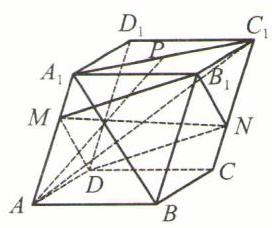
\includegraphics[width=0.2\textwidth]{bodyxb/src/bo_d20cdrf7aajc73bfmvhg_181_1158_1103_272_228_0.jpg}
\end{center}


(第 30 题)

(2)当 $\dfrac{A{A}_{1}}{AB} = 1$ 时, $A{C}_{1} \bot  {A}_{1}B$ ,理由如下,

设 $\vv{A{A}_{1}} = c,\vv{AD} = b,\vv{AB} = a$ ,且 $c$ 与 $b,c$ 与 $a,b$ 与 $a$ 的夹角均为 ${60}^{ \circ  }$ .

$\because$ 底面 ${ABCD}$ 为菱形, $\therefore \left| \vv{b}\right|  = \left| \vv{a}\right|$ .

$\because \vv{A{C}_{1}} = \vv{A{A}_{1}} + \vv{{A}_{1}{C}_{1}} = \vv{{A}_{1}{B}_{1}} + \vv{{A}_{1}{D}_{1}} + \vv{A{A}_{1}} = a + b + c,\vv{{A}_{1}B} = \vv{{A}_{1}A} + \vv{AB} = a - c$ ,

若 $A{C}_{1} \bot  {A}_{1}B$ ,则 $\vv{A{C}_{1}} \bot  \vv{{A}_{1}B}$ ,即 $\vv{A{C}_{1}} \cdot  \vv{{A}_{1}B} = \left( {a + c + b}\right)  \cdot  \left( {a - c}\right)  = {a}^{2} - {c}^{2} + a \cdot  b - c \cdot  b = 0$ ,

即 ${\left| a\right| }^{2} - {\left| c\right| }^{2} + \left| a\right|  \cdot  \left| b\right| \cos {60}^{ \circ  } - \left| c\right|  \cdot  \left| b\right| \cos {60}^{ \circ  } = {\left| a\right| }^{2} - {\left| c\right| }^{2} + \dfrac{1}{2}{\left| a\right| }^{2} - \dfrac{1}{2}\left| c\right|  \cdot  \left| a\right|  = 0$ ,

解得 $\left| \vv{a}\right|  = \left| \mathbf{c}\right|$ 或 $3\left| \vv{a}\right|  + 2\left| \mathbf{c}\right|  = 0$ 舍,所以 $\dfrac{A{A}_{1}}{AB} = 1$ 时, $A{C}_{1} \bot  {A}_{1}B$ .

) $\because \vv{{A}_{1}P} = \dfrac{1}{2}\vv{{A}_{1}{C}_{1}},\;\therefore \;\vv{AP} = \vv{A{A}_{1}} + \dfrac{1}{2}\vv{{A}_{1}{C}_{1}} = \vv{A{A}_{1}} + \dfrac{1}{2}\vv{AB} + \dfrac{1}{2}\vv{AD}$ .

$\because {AB} = {A{A}_{1}} = 1,\;\therefore \;{\vv{AP}}^{2} = {\left( \vv{A{A}_{1}} + \dfrac{1}{2}\vv{AB} + \dfrac{1}{2}\vv{AD}\right) }^{2} = {\vv{A{A}_{1}}}^{2} + \dfrac{1}{4}{\vv{AB}}^{2} + \dfrac{1}{4}{\vv{AD}}^{2} + \vv{A{A}_{1}} \cdot  \vv{AB} + \vv{A{A}_{1}} \cdot  \vv{AD} +$

$\dfrac{1}{2}\vv{AB} \cdot  \vv{AD} = 1 + \dfrac{1}{4} + \dfrac{1}{4} + \dfrac{1}{2} + \dfrac{1}{2} + \dfrac{1}{4} = \dfrac{11}{4},$

$\therefore \left| \vv{AP}\right|  = \dfrac{\sqrt{11}}{2},\;\therefore \;{AP}$ 的长为 $\dfrac{\sqrt{11}}{2}$ .

31. D

32. $B$

33. $C$ 提示: 向量 $\vv{a}$ 在 $\vv{b}$ 上的投影向量为 $\dfrac{\vv{a} \cdot  \vv{b}}{\left| \vv{b}\right| }\dfrac{\vv{b}}{\left| \vv{b}\right| } = \dfrac{\left( {2,2,1}\right)  \cdot  \left( {1,1,0}\right) }{\sqrt{2}} \times  \dfrac{\left( 1,1,0\right) }{\sqrt{2}} = 2\left( {1,1,0}\right)  = \left( {2,2,0}\right)$ .

34. D 提示: $\mathbf{k}\vv{a} + \vv{b} = k\left( {1,1,0}\right)  + \left( {-1,0, - 2}\right)  = \left( {k - 1,k, - 2}\right) ,2\vv{a} - \vv{b} = 2\left( {1,1,0}\right)  - \left( {-1,0, - 2}\right)  = \left( {3,2,2}\right)$ .

由 ${ka} + b$ 与 ${2a} - b$ 互相垂直,得 $\left( {k - 1,k, - 2}\right)  \cdot  \left( {3,2,2}\right)  = 0$ ,即 ${5k} - 7 = 0$ ,所以 $k = \dfrac{7}{5}$ .

35. D 提示: 由 $a \bot  c$ ,得 $a \cdot  c = 0$ ,即 $x - 4 + 2 = 0$ ,解得 $x = 2$ .

由 $\vv{b}//\mathbf{c}$ ,得 $\dfrac{1}{2} = \dfrac{y}{-4} = \dfrac{z}{2}$ ,解得 $y =  - 2,z = 1$ . 所以 $\left| {2\vv{a} + \vv{b}}\right|  = \left| {2\left( {1,1,1}\right)  + \left( {1, - 2,1}\right) }\right|  = \left| \left( {3,0,3}\right) \right|  = 3\sqrt{2}$ .

36. A 提示: 因为 $\vv{a},\vv{b},\mathbf{c}$ 共面,可设 $\mathbf{c} = x\vv{a} + y\vv{b}$ ,即 $\left( {1,4,\lambda }\right)  = x\left( {3, - 1,2}\right)  + y\left( {4,3, - 2}\right)$ ,

得 $\left\{  \begin{array}{l} 1 = {3x} + {4y}, \\  4 =  - x + {3y}, \\  \lambda  = {2x} - {2y}, \end{array}\right.$ 解得 $\left\{  \begin{array}{l} x =  - 1, \\  y = 1, \\  \lambda  =  - 4. \end{array}\right.$

37. A 提示: 因为 $\vv{a} = \left( {2,4,x}\right) ,\vv{b} = \left( {2,y,2}\right)$ ,且 $\left| \vv{a}\right|  = 6,\vv{a}\bot \vv{b}$ ,

所以 $\left\{  \begin{array}{l} \left| \vv{a}\right|  = \sqrt{{2}^{2} + {4}^{2} + {x}^{2}} = 6, \\  \vv{a} \cdot  \vv{b} = 4 + {4y} + {2x} = 0, \end{array}\right.$ 解得 $\left\{  \begin{array}{l} x = 4, \\  y =  - 3 \end{array}\right.$ 或 $\left\{  \begin{array}{l} x =  - 4, \\  y = 1, \end{array}\right.$ 所以 $x + y = 1$ 或 $x + y =  - 3$ .

38. D 提示: 由题意得 $a \cdot  b < 0$ 且 $a$ 与 $b$ 不反向,由 $a \cdot  b < 0$ ,得 $- 1 \times  1 - 2\left( {x - 1}\right)  - 1 \times  1 < 0$ ,解得 $x > 0$ .

若 $\vv{a}$ 与 $\vv{b}$ 反向,设 $\vv{b} = t\vv{a}\left( {t < 0}\right)$ ,则 $\left\{  \begin{array}{l}  - 1 = t, \\  x - 1 =  - {2t}, \end{array}\right.$ 解得 $\left\{  \begin{array}{l} t =  - 1, \\  x = 3. \end{array}\right.$

综上可得, $x$ 的取值范围是 $\left( {0,3}\right)  \cup  \left( {3, + \infty }\right)$ .

39. C 提示: 显然 $\vv{a}$ 与 $\vv{b}$ 不平行,设平面 $\alpha$ 的法向量为 $\mathbf{n} = \left( {x,y,z}\right)$ ,

则 $\left\{  \begin{array}{l} \vv{a} \cdot  \mathbf{n} = 0, \\  \vv{b} \cdot  \mathbf{n} = 0, \end{array}\right.$ 所以 $\left\{  \begin{array}{l} {2x} + {3y} + z = 0, \\  {5x} + {6y} + {4z} = 0. \end{array}\right.$ 令 $z = 1$ ,得 $x =  - 2,y = 1$ . 所以 $\mathbf{n} = \left( {-2,1,1}\right)$ .

40. A 提示: 设 $l$ 与 $\alpha$ 所成角的大小为 $\theta$ ,

则 $\sin \theta  = \left| {\cos \langle u,n\rangle }\right|  = \dfrac{\left| u \cdot  n\right| }{\left| u\right|  \cdot  \left| n\right| } = \dfrac{\left| 0 \times  1 + 0 \times  \left( -1\right)  + 1 \times  1\right| }{\sqrt{1 + 1} \times  \sqrt{1 + 1}} = \dfrac{1}{2}$ ,故 $l$ 与 $\alpha$ 所成角的正弦值为 $\dfrac{1}{2}$ .

41. D 提示: 设两条异面直线所成的角为 $\theta$ ,

且这两条异面直线的方向向量分别是 $\vv{OC} = \left( {-1,0, - 1}\right) ,\vv{AB} = \left( {-2,1,1}\right)$ ,

则 $\cos \theta  = \left| \dfrac{\vv{OC} \cdot  \vv{AB}}{\left| \vv{OC}\right|  \cdot  \left| \vv{AB}\right| }\right|  = \left| \dfrac{\left( {-1}\right)  \times  \left( {-2}\right)  + 0 \times  1 + \left( {-1}\right)  \times  1}{\sqrt{{\left( -1\right) }^{2} + {0}^{2} + {\left( -1\right) }^{2}} \cdot  \sqrt{{\left( -2\right) }^{2} + {1}^{2} + {1}^{2}}}\right|  = \dfrac{\sqrt{3}}{6}$ ,且 $0 < \theta  \leq  \dfrac{\pi }{2}$ , 所以 $\sin \theta  = \sqrt{1 - {\cos }^{2}\theta } = \dfrac{\sqrt{33}}{6}$ ,即异面直线 ${OC}$ 与 ${AB}$ 所成角的正弦值为 $\dfrac{\sqrt{33}}{6}$ .

42. $B$ 提示: 如图,以 $D$ 为坐标原点, ${DA},{DC},D{D}_{1}$ 分别为 $x,y,z$ 轴,建立空间直角坐标系. 设正方体的棱长为 2,

\begin{center}
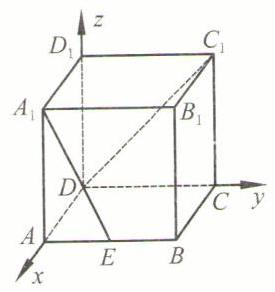
\includegraphics[width=0.2\textwidth]{bodyxb/src/bo_d20cdrf7aajc73bfmvhg_182_1217_1359_275_292_0.jpg}
\end{center}


(第 42 题)

则 ${A}_{1}\left( {2,0,2}\right) ,E\left( {2,1,0}\right) ,D\left( {0,0,0}\right) ,{C}_{1}\left( {0,2,2}\right)$ ,

可得 $\vv{{A}_{1}E} = \left( {0,1, - 2}\right) ,\vv{D{C}_{1}} = \left( {0,2,2}\right)$ .

则 $\cos \left\langle  {\vv{{A}_{1}E},\vv{D{C}_{1}}}\right\rangle   = \dfrac{\vv{{A}_{1}E} \cdot  \vv{D{C}_{1}}}{\left| \vv{{A}_{1}E}\right|  \cdot  \left| \vv{D{C}_{1}}\right| } = \dfrac{-2}{\sqrt{5} \times  2\sqrt{2}} =  - \dfrac{\sqrt{10}}{10}$ ,

所以直线 ${A}_{1}E,{C}_{1}D$ 所成角的余弦值为 $\dfrac{\sqrt{10}}{10}$ .

43. B 提示: 设正方体的棱长为 4,直线 ${D}_{1}E$ 与平面 ${AC}{D}_{1}$ 所成的角为 $\alpha$ ,以 ${DA},{DC},D{D}_{1}$ 所在直线为 $x,y,z$ 轴,建立空间直角坐标系.

\begin{center}
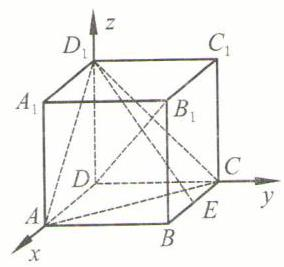
\includegraphics[width=0.2\textwidth]{bodyxb/src/bo_d20cdrf7aajc73bfmvhg_182_1207_1726_284_267_0.jpg}
\end{center}


(第 43 题)

${B}_{1}\left( {4,4,4}\right) ,{D}_{1}\left( {0,0,4}\right) ,A\left( {4,0,0}\right) ,C\left( {0,4,0}\right) ,E\left( {2,4,0}\right) ,\vv{A{D}_{1}} = \left( {-4,0,4}\right) ,\vv{C{D}_{1}} =$  $\left( {0, - 4,4}\right) ,\vv{D{B}_{1}} \cdot  \vv{A{D}_{1}} = 0,\vv{D{B}_{1}} \cdot  \vv{C{D}_{1}} = 0$ ,所以 $D{B}_{1} \bot  A{D}_{1},D{B}_{1} \bot  C{D}_{1}$ .

由于 $A{D}_{1},C{D}_{1}$ 为平面 ${ABC}{D}_{1}$ 内两相交直线,所以 $D{B}_{1} \bot$ 平面 ${AC}{D}_{1}$ ,

即平面 ${AC}{D}_{1}$ 的法向量为 $\vv{D{B}_{1}} = \left( {4,4,4}\right)$ ,又因为 $\vv{{D}_{1}E} = \left( {2,4, - 4}\right)$ ,

所以 $\sin \alpha  = \dfrac{\left| \vv{{D}_{1}E} \cdot  \vv{D{B}_{1}}\right| }{\left| \vv{{D}_{1}E}\right|  \cdot  \left| \vv{D{B}_{1}}\right| } = \dfrac{\sqrt{3}}{9}$ .

44. A 提示: 设平面 ${ABCD}$ 的法向量为 $\mathbf{n} = \left( {x,y,z}\right)$ ,

则有 $\left\{  \begin{array}{l} \mathbf{n} \cdot  \vv{AB} = {4x} - {2y} + {3z} = 0 \\  \mathbf{n} \cdot  \vv{AD} =  - {4x} + y = 0 \end{array}\right.$ ,令 $x = 3$ ,则 $y = {12},z = 4$ ,

即 $\mathbf{n} = \left( {3,{12},4}\right)$ ,所以顶点 $S$ 到底面 ${ABCD}$ 的距离为 $\left| \dfrac{\mathbf{n} \cdot  \vv{AS}}{\left| \mathbf{n}\right| }\right|  = \left| \dfrac{-9 + {12} - {16}}{13}\right|  = 1$ .

45. A 提示: $\vv{BC} = \left( {-4,2,0}\right) ,\dfrac{\vv{BC}}{\left| \vv{BC}\right| } = \left( {-\dfrac{2\sqrt{5}}{5},\dfrac{\sqrt{5}}{5},0}\right) ,\vv{BA} = \left( {0, - 1, - 3}\right) ,A$ 到直线 ${BC}$ 的距离为 $d = \sqrt{\vv{B{A}^{2}} - {\left( \vv{BA} \cdot  \dfrac{\vv{BC}}{\left| \vv{BC}\right| }\right) }^{2}} =$  $\sqrt{{10} - {\left( -\dfrac{\sqrt{5}}{5}\right) }^{2}} = \dfrac{7\sqrt{5}}{5}.$ 46. 2 47. -8 48. $\sqrt{2}$ 49. $\left( {\dfrac{2}{3},\dfrac{2}{3}, - \dfrac{1}{3}}\right)$ 50. 1 51. 12 提示: 点 $A\left( {2, - 1,3}\right)$ 关于平面 ${xOz}$ 的对称点为 $B\left( {2,1,3}\right)$ ,则 $\vv{OA} = \left( {2, - 1,3}\right) ,\vv{OB} = \left( {2,1,3}\right)$ , 所以 $\vv{OA} \cdot  \vv{OB} = \left( {2, - 1,3}\right)  \cdot  \left( {2,1,3}\right)  = {12}$ . 52. $\sqrt{37}$ 提示:由题意知 $\left| \vv{b}\right|  = \sqrt{{1}^{2} + {2}^{2} + {\left( -2\right) }^{2}} = 3$ ,故 $\left| {2\vv{a} - \vv{b}}\right|  = \sqrt{4{\left| \vv{a}\right| }^{2} - 4\vv{a} \cdot  \vv{b} + {\left| \vv{b}\right| }^{2}} = \sqrt{37}$ .

53.(-1,1,0)提示:因为 $\left| \vv{a}\right| \cos \langle \vv{a},\vv{b}\rangle  = \dfrac{\vv{a} \cdot  \vv{b}}{\left| \vv{b}\right| } = \dfrac{-2}{\sqrt{2}} =  - \sqrt{2}$ ,又 $\dfrac{\vv{b}}{\left| \vv{b}\right| } = \dfrac{\sqrt{2}}{2}\vv{b}$ ,

所以 $a$ 在 $b$ 方向上的投影向量为 $\left| a\right| \cos \langle a,b\rangle  \cdot  \dfrac{b}{\left| b\right| } =  - b = \left( {-1,1,0}\right)$ .

54. -30 提示: 由题意得, $\vv{AP} = \left( {-2,a - 2,b + 1}\right) ,\vv{AB} = \left( {1, - 2,2}\right)$ .

因为点 $P$ 在直线 ${AB}$ 上运动,则存在实数 $\lambda$ ,使得 $\vv{AP} = \lambda \vv{AB}$ ,则 $\left\{  \begin{array}{l}  - 2 = \lambda , \\  a - 2 =  - {2\lambda }, \\  b + 1 = {2\lambda }, \end{array}\right.$

解得 $\left\{  \begin{array}{l} \lambda  =  - 2, \\  a = 6, \\  b =  - 5, \end{array}\right.$ 故 ${ab} =  - {30}$ .

55. -2 提示: $\vv{AB} = \left( {0,1, - 1}\right) ,\vv{AC} = \left( {1,0, - 1}\right)$ ,

因为点 $P\left( {x,1,2}\right)$ 在平面 ${ABC}$ 上,所以存在 $m,n$ 使得 $\vv{AP} = m\vv{AB} + n\vv{AC}$ .

即 $\left( {x,1,1}\right)  = m\left( {0,1, - 1}\right)  + n\left( {1,0, - 1}\right)$ ,故 $\left\{  \begin{array}{l} x = n, \\  1 = m, \\  1 =  - m - n, \end{array}\right.$ 解得 $x =  - 2$ .

56. $\dfrac{\sqrt{6}}{6}$ 提示: 建立如图所示的空间直角坐标系,

\begin{center}
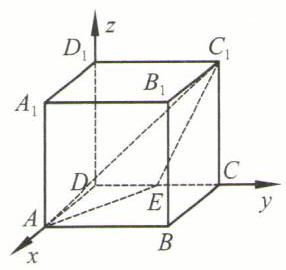
\includegraphics[width=0.2\textwidth]{bodyxb/src/bo_d20cdrf7aajc73bfmvhg_183_1144_1382_286_270_0.jpg}
\end{center}


(第 56 题)

则 $A\left( {1,0,0}\right) ,{C}_{1}\left( {0,1,1}\right) ,E\left( {0,\dfrac{1}{2},0}\right) ,{A}_{1}\left( {1,0,1}\right)$ .

设平面 ${AE}{C}_{1}$ 的一个法向量为 $\mathbf{n} = \left( {x,y,z}\right)$ ,

$\vv{AE} = \left( {-1,\dfrac{1}{2},0}\right) ,\vv{E{C}_{1}} = \left( {0,\dfrac{1}{2},1}\right) ,\vv{A{A}_{1}} = \left( {0,0,1}\right)$ ,则 $\left\{  \begin{array}{l} \mathbf{n} \cdot  \vv{AE} =  - x + \dfrac{1}{2}y = 0, \\  \mathbf{n} \cdot  \vv{E{C}_{1}} = \dfrac{1}{2}y + z = 0, \end{array}\right.$ 令 $y = 2$ ,

则 $\mathbf{n} = \left( {1,2, - 1}\right)$ .

设点 ${A}_{1}$ 到平面 ${AE}{C}_{1}$ 的距离为 $d$ ,则 $d = \dfrac{\left| \vv{A{A}_{1}} \cdot  n\right| }{\left| n\right| } = \dfrac{1}{\sqrt{6}} = \dfrac{\sqrt{6}}{6}$ ,即点 ${A}_{1}$ 到平面 ${AE}{C}_{1}$ 的距离为 $\dfrac{\sqrt{6}}{6}$ . 57. $\dfrac{\sqrt{5}}{5}$ 提示:如图建立空间直角坐标系, $C$ 为底面圆周上一点,则 $\angle {ACB} = {90}^{ \circ  }$ .

又 ${AC} = \sqrt{3},{AB} = {PC} = 2$ ,

$\therefore {BC} = 1,{PO} = \sqrt{3}$ .

$\therefore A\left( {0, - 1,0}\right) ,B\left( {0,1,0}\right) ,P\left( {0,0,\sqrt{3}}\right) ,C\left( {\dfrac{\sqrt{3}}{2},\dfrac{1}{2},0}\right) ,\vv{PB} = \left( {0,1, - \sqrt{3}}\right) ,\vv{PC} = \left( {\dfrac{\sqrt{3}}{2},\dfrac{1}{2}, - \sqrt{3}}\right)$ ,

设平面 ${CPB}$ 的一个法向量为 $\mathbf{m} = \left( {x,y,z}\right)$ . 则 $\left\{  \begin{array}{l} \mathbf{m} \cdot  \vv{PB} = 0, \\  \mathbf{m} \cdot  \vv{PC} = 0, \end{array}\right.$

即 $\left\{  \begin{array}{l} y - \sqrt{3}z = 0, \\  \dfrac{\sqrt{3}}{2}x + \dfrac{1}{2}y - \sqrt{3}z = 0, \end{array}\right.$ 令 $z = 1$ ,得 $x = 1,y = \sqrt{3},\;\therefore \;m = \left( {1,\sqrt{3},1}\right)$ .

\begin{center}
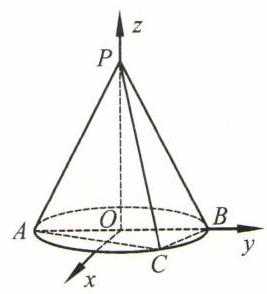
\includegraphics[width=0.2\textwidth]{bodyxb/src/bo_d20cdrf7aajc73bfmvhg_184_1213_137_267_294_0.jpg}
\end{center}


(第 57 题)

又因为平面 ${APB}$ 的一个法向量为 $\mathbf{n} = \left( {1,0,0}\right) ,\therefore \cos \langle \mathbf{m},\mathbf{n}\rangle  = \dfrac{\mathbf{m} \cdot  \mathbf{n}}{\left| \mathbf{m}\right| \left| \mathbf{n}\right| } = \dfrac{1}{\sqrt{1 + 3 + 1} \times  1}$  $= \dfrac{1}{\sqrt{5}} = \dfrac{\sqrt{5}}{5}$ ,于是锐二面角 $A - {PB} - C$ 的余弦值为 $\dfrac{\sqrt{5}}{5}$ .

58. (1) 依题意可得 $A\left( {0,0,0}\right) ,B\left( {1,0,0}\right) ,C\left( {0,\sqrt{2},0}\right) ,{A}_{1}\left( {0,0,2}\right) ,{B}_{1}\left( {1,0,2}\right) ,{C}_{1}\left( {0,\sqrt{2},2}\right)$ , $D\left( {0,\sqrt{2},1}\right)$ ,则 $\vv{{A}_{1}C} = \left( {0,\sqrt{2}, - 2}\right) ,\vv{BD} = \left( {-1,\sqrt{2},1}\right)$ ,所以 $\vv{{A}_{1}C} \cdot  \vv{BD} = 0 \times  \left( {-1}\right)  + \sqrt{2}$  $\times  \sqrt{2} - 2 \times  1 = 0$ ,所以 ${A}_{1}C \bot  {BD}$ .

(2)因为 $\vv{{A}_{1}C} = \left( {0,\sqrt{2}, - 2}\right) ,\vv{AC} = \left( {0,\sqrt{2},0}\right) ,\vv{A{B}_{1}} = \left( {1,0,2}\right)$ .

设平面 $A{B}_{1}C$ 的法向量为 $\mathbf{n} = \left( {x,y,z}\right)$ ,则 $\left\{  \begin{array}{l} \mathbf{n} \cdot  \vv{A{B}_{1}} = x + {2z} = 0, \\  \mathbf{n} \cdot  \vv{AC} = \sqrt{2}y = 0. \end{array}\right.$

令 $z =  - 1$ ,可得 $x = 2,y = 0$ ,此时 $\mathbf{n} = \left( {2,0, - 1}\right)$ .

设直线 ${A}_{1}C$ 与平面 $A{B}_{1}C$ 所成角为 $\theta$ ,则 $\sin \theta  = \dfrac{\left| \vv{{A}_{1}C} \cdot  n\right| }{\left| \vv{{A}_{1}C}\right|  \cdot  \left| n\right| } = \dfrac{2}{\sqrt{6} \times  \sqrt{5}} = \dfrac{\sqrt{30}}{15}$ ,所以直线 ${A}_{1}C$ 与平面 $A{B}_{1}C$ 所成角的正弦值为 $\dfrac{\sqrt{30}}{15}$ .

(3) 由 (2)知 $\vv{{A}_{1}C} = \left( {0,\sqrt{2}, - 2}\right) ,n = \left( {2,0, - 1}\right)$ 为平面 $A{B}_{1}C$ 的一个法向量,所以点 ${A}_{1}$ 到平面 $A{B}_{1}C$ 的距离

$d = \dfrac{\left| \vv{{A}_{1}C} \cdot  \mathbf{n}\right| }{\left| \mathbf{n}\right| } = \dfrac{2}{\sqrt{5}} = \dfrac{2\sqrt{5}}{5}.$

59. 以点 $A$ 为原点,分别以向量 $\vv{AB},\vv{AC}$ 与 $\vv{A{A}_{1}}$ 的方向为 $x,y$ 与 $z$ 轴的正方向,建立空间直角坐标系,可得有关点的坐标分别为 $B\left( {2,0,0}\right) ,C\left( {0,2,0}\right) ,{A}_{1}\left( {0,0,2}\right) ,{C}_{1}\left( {0,2,2}\right) ,E\left( {0,2,1}\right) ,F\left( {1,1,0}\right)$ .

(1) $\vv{{A}_{1}B} = \left( {2,0, - 2}\right) ,\vv{EF} = \left( {1, - 1, - 1}\right) ,\cos \left\langle  {\vv{{A}_{1}B},\vv{EF}}\right\rangle   = \dfrac{\vv{{A}_{1}B} \cdot  \vv{EF}}{\left| \vv{{A}_{1}B}\right| \left| \vv{EF}\right| } = \dfrac{\sqrt{6}}{3}$ .

因此,直线 ${A}_{1}B$ 与直线 ${EF}$ 所成角的大小为 $\arccos \dfrac{\sqrt{6}}{3}$ .

(2) $\vv{AE} = \left( {0,2,1}\right) ,\vv{AF} = \left( {1,1,0}\right)$ . 设 $n = \left( {x,y,z}\right)$ 是平面 ${AEF}$ 的一个法向量,有 $\left\{  \begin{array}{l} n \cdot  \vv{AE} = {2y} + z = 0, \\  n \cdot  \vv{AF} = x + y = 0. \end{array}\right.$ 不妨取 $y =  - 1$ , 从而得到平面 ${AEF}$ 的一个法向量 $n = \left( {1, - 1,2}\right)$ ,易知 $\vv{AC} = \left( {0,2,0}\right)$ 为平面 ${AB}{A}_{1}$ 的一个法向量,从而 $\left| {\cos \langle \mathbf{n},\vv{AC}\rangle }\right|  = \dfrac{\left| \mathbf{n} \cdot  \vv{AC}\right| }{\left| \mathbf{n}\right| \left| \vv{AC}\right| } = \dfrac{\sqrt{6}}{6}.$

因此,平面 ${AB}{A}_{1}$ 与平面 ${AEF}$ 所成的锐二面角的大小为 $\arccos \dfrac{\sqrt{6}}{6}$ .

\begin{center}
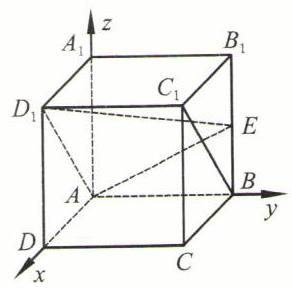
\includegraphics[width=0.2\textwidth]{bodyxb/src/bo_d20cdrf7aajc73bfmvhg_184_1203_1477_292_289_0.jpg}
\end{center}


(第 60 题)

60. 如图,以 $A$ 为坐标原点,分别以 $\vv{AD},\vv{AB}$ 与 $\vv{A{A}_{1}}$ 为 $x,y$ 与 $z$ 轴正方向,建立空间直角坐标系,设正方体 ${ABCD} - {A}_{1}{B}_{1}{C}_{1}{D}_{1}$ 的棱长为 2,则 ${A}_{1}\left( {0,0,2}\right) ,{D}_{1}\left( {2,0,2}\right) ,E\left( {0,2,1}\right)$ ,

$\vv{A{D}_{1}} = \left( {2,0,2}\right) ,\vv{AE} = \left( {0,2,1}\right) ,\vv{B{C}_{1}} = \left( {2,0,2}\right)$ .

(1) 设平面 $A{D}_{1}E$ 的法向量为 $\mathbf{n} = \left( {x,y,z}\right)$ ,由 $\left\{  \begin{array}{l} \mathbf{n} \cdot  \vv{A{D}_{1}} = 0, \\  \mathbf{n} \cdot  \vv{AE} = 0, \end{array}\right.$ 得 $\left\{  \begin{array}{l} {2x} + {2z} = 0, \\  {2y} + z = 0, \end{array}\right.$ 令 $z =  - 2$ ,得 $x = 2,y = 1$ ,则 $\mathbf{n} = \left( {2,1, - 2}\right)$ . 因为 $\vv{B{C}_{1}} \cdot  \mathbf{n} = 2 \times  2 + 0 \times  1 + 2 \times  \left( {-2}\right)  = 0$ ,且 $B{C}_{1}$ 在平面 $A{D}_{1}E$ 外,

所以 $B{C}_{1}//$ 平面 $A{D}_{1}E$ .

(2)设直线 $A{A}_{1}$ 与平面 $A{D}_{1}E$ 所成角为 $\theta$ ,由(1)知平面 $A{D}_{1}E$ 的法向量 $n = \left( {2,1, - 2}\right)$ ,又 $\vv{A{A}_{1}} = \left( {0,0,2}\right)$ ,

所以 $\sin \theta  = \dfrac{\left| \mathbf{n} \cdot  \vv{A{A}_{1}}\right| }{\left| \mathbf{n}\right|  \cdot  \left| \vv{A{A}_{1}}\right| } = \dfrac{4}{3 \times  2} = \dfrac{2}{3}$ .

61. 以 $D$ 为原点,分别以向量 $\vv{DA},\vv{DC}$ 与 $\vv{D{D}_{1}}$ 的方向为 $x,y$ 与 $z$ 轴的正方向,建立空间直角坐标系,可得有关点的坐标分别为 $B\left( {1,2,0}\right) ,C\left( {0,2,0}\right) ,{D}_{1}\left( {0,0,2}\right) ,H\left( {0,1,2}\right) ,F\left( {1,2,1}\right)$ .

(1) $\vv{HF} = \left( {1,1, - 1}\right)$ . 在长方体 ${ABCD} - {A}_{1}{B}_{1}{C}_{1}{D}_{1}$ 中,易知 $D{D}_{1} \bot$ 平面 ${ABCD}$ ,故 $m = \left( {0,0,1}\right)$ 为平面 ${ABCD}$ 的一个

法向量. 设直线 ${HF}$ 与平面 ${ABCD}$ 所成角的大小为 $\theta$ ,则 $\sin \theta  = \dfrac{\left| m \cdot  \vv{HF}\right| }{\left| m\right| \left| \vv{HF}\right| } = \dfrac{\sqrt{3}}{3}$ ,故直线 ${HF}$ 与平面 ${ABCD}$ 所成角的大小为 $\arcsin \dfrac{\sqrt{3}}{3}$ .

(2) $\vv{C{D}_{1}} = \left( {0, - 2,2}\right) ,\vv{BC} = \left( {-1,0,0}\right)$ .

设 $\mathbf{n} = \left( {x,y,z}\right)$ 是平面 ${A}_{1}{BC}{D}_{1}$ 的一个法向量,有 $\left\{  \begin{array}{l} \mathbf{n} \cdot  \vv{C{D}_{1}} =  - {2y} + {2z} = 0, \\  \mathbf{n} \cdot  \vv{BC} =  - x = 0. \end{array}\right.$

不妨取 $z = 1$ ,从而得到平面 ${A}_{1}{BC}{D}_{1}$ 的一个法向量 $\mathbf{n} = \left( {0,1,1}\right)$ .

假设线段 ${HF}$ 上存在满足题意的点 $Q$ ,设 $\vv{HQ} = \lambda \vv{HF},\lambda  \in  \left\lbrack  {0,1}\right\rbrack$ .

可求得 $Q$ 点坐标为 $\left( {\lambda ,\lambda  + 1,2 - \lambda }\right) ,\vv{{D}_{1}Q} = \left( {\lambda ,\lambda  + 1, - \lambda }\right)$ .

点 $Q$ 到平面 ${A}_{1}{BC}{D}_{1}$ 的距离为 $\dfrac{\left| \vv{D{Q}_{1}} \cdot  \mathbf{n}\right| }{\left| \mathbf{n}\right| } = \dfrac{\sqrt{2}}{2}$ .

因为 $\dfrac{\sqrt{2}}{2} < \sqrt{2}$ ,所以线段 ${HF}$ 上不存在满足题意的点 $Q$ .

62. (1) 证明: 因为 ${PA}$ 是圆柱的母线,所以 ${PA} \bot$ 平面 ${ABCD}$ ,而 ${CD} \subset$ 平面 ${ABCD}$ ,

\begin{center}
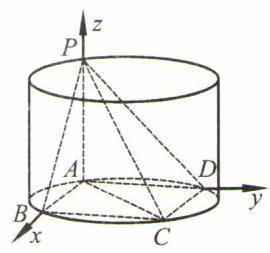
\includegraphics[width=0.2\textwidth]{bodyxb/src/bo_d20cdrf7aajc73bfmvhg_185_1141_714_270_253_0.jpg}
\end{center}


(第 62 题)

所以 ${PA} \bot  {CD}$ . 因为底面 ${ABCD}$ 是圆柱底面圆的内接矩形,所以 ${AC}$ 是直径,从而 ${CD}$  $\bot  {AD}$ ,

又因为 ${PA} \cap  {AD} = A,{PA} \subset$ 平面 ${PAD},{AD} \subset$ 平面 ${PAD}$ ,所以 ${CD} \bot$ 平面 ${PAD}$ ,

而 ${CD} \subset$ 平面 ${PCD}$ ,所以平面 ${PCD} \bot$ 平面 ${PAD}$ .

(2)由题意 ${PA}\bot$ 平面 ${ABCD},{AB}\bot {AD}$ ,又 ${AB} \subset$ 平面 ${ABCD}$ , ${AD} \subset$ 平面 ${ABCD}$ ,

所以 ${AP} \bot  {AB},{AP} \bot  {AD}$ ,所以 ${AB},{AD},{AP}$ 两两互相垂直.

如图,以 $A$ 为原点,分别以 $\vv{AB},\vv{AD}$ 与 $\vv{AP}$ 为 $x,y$ 与 $z$ 轴的正方向,建立空间直角坐标系,则 $A\left( {0,0,0}\right) ,B\left( {1,0,0}\right) ,C\left( {1,2,0}\right) ,D\left( {0,2,0}\right) ,P\left( {0,0,2}\right)$ ,

所以 $\vv{PB} = \left( {1,0, - 2}\right) ,\vv{PC} = \left( {1,2, - 2}\right) ,\vv{PD} = \left( {0,2, - 2}\right)$ .

设 $\mathbf{m} = \left( {{x}_{1},{y}_{1},{z}_{1}}\right)$ 为平面 ${PBC}$ 的法向量,则 $\left\{  \begin{array}{l} \mathbf{m} \cdot  \vv{PB} = {x}_{1} - 2{z}_{1} = 0, \\  \mathbf{m} \cdot  \vv{PC} = {x}_{1} + 2{y}_{1} - 2{z}_{1} \end{array}\right.$

令 ${z}_{1} = 1$ ,可得 ${x}_{1} = 2,{y}_{1} = 0$ ,得平面 ${PBC}$ 的一个法向量为 $m = \left( {2,0,1}\right)$ .

设 $\mathbf{n} = \left( {{x}_{2},{y}_{2},{z}_{2}}\right)$ 为平面 ${PCD}$ 的法向量,则 $\left\{  \begin{array}{l} \mathbf{n} \cdot  \vv{PD} = 2{y}_{2} - 2{z}_{2} = 0, \\  \mathbf{n} \cdot  \vv{PC} = {x}_{2} + 2{y}_{2} - 2{z}_{2} = 0. \end{array}\right.$

令 ${y}_{2} = 1$ ,可得 ${x}_{2} = 0,{z}_{2} = 1$ ,得平面 ${PCD}$ 的一个法向量 $n = \left( {0,1,1}\right)$ .

设平面 ${PBC}$ 与平面 ${PCD}$ 所成的锐二面角为 $\theta$ ,则 $\cos \theta  = \dfrac{\left| \mathbf{m} \cdot  \mathbf{n}\right| }{\left| \mathbf{m}\right| \left| \mathbf{n}\right| } = \dfrac{1}{\sqrt{5} \times  \sqrt{2}} = \dfrac{\sqrt{10}}{10}$ ,

所以平面 ${PBC}$ 与平面 ${PCD}$ 所成的锐二面角的余弦值为 $\dfrac{\sqrt{10}}{10}$ .

63. A 提示: 设 ${A}_{i}\left( {{x}_{i},{y}_{i},{z}_{i}}\right) ,M\left( {x,y,z}\right)$ ,由 $\mathop{\sum }\limits_{{i = 1}}^{n}\left( {i\vv{M{A}_{i}}}\right)  = \mathbf{0}$ ,得 $\mathop{\sum }\limits_{{i = 1}}^{n}i\left( {{x}_{i} - x,{y}_{i} - y,{z}_{i} - z}\right)  = \mathbf{0}$ ,

所以 $\mathop{\sum }\limits_{{i = 1}}^{n}i\left( {{x}_{i} - x}\right)  = 0,\mathop{\sum }\limits_{{i = 1}}^{n}i\left( {{y}_{i} - y}\right)  = 0,\mathop{\sum }\limits_{{i = 1}}^{n}i\left( {{z}_{i} - z}\right)  = 0$ ,

所以 $x = \dfrac{2\mathop{\sum }\limits_{{i = 1}}^{n}i{x}_{i}}{n\left( {n + 1}\right) },y = \dfrac{2\mathop{\sum }\limits_{{i = 1}}^{n}i{y}_{i}}{n\left( {n + 1}\right) },z = \dfrac{2\mathop{\sum }\limits_{{i = 1}}^{n}i{z}_{i}}{n\left( {n + 1}\right) }$ ,

所以满足条件的点 $M$ 的个数为 1 个.

64. A 提示: 由题设知: 平面 $\alpha$ 的法向量 $m = \left( {2, - 3, - 1}\right)$ ,直线 $l$ 的方向向量 $n = \left( {-1,2, - 3}\right)$ ,

且平面 $\alpha$ 与直线 $l$ 相交于(0,0,0),所以直线 $l$ 与平面 $\alpha$ 所成角的正弦值为 $\left| {\cos \langle m,n\rangle }\right|  = \dfrac{\left| m \cdot  n\right| }{\left| m\right| \left| n\right| } = \dfrac{5}{\sqrt{14} \times  \sqrt{14}} = \dfrac{5}{14}$ .

65. $B$ 提示: 在正四棱柱 ${ABCD} - {A}_{1}{B}_{1}{C}_{1}{D}_{1}$ 中, $E,F$ 分别为侧面 ${AB}{B}_{1}{A}_{1}$ 和侧面 ${BC}{C}_{1}{B}_{1}$ 的中心, $G$ 为 $B{B}_{1}$ 的中点, $N$ 为 2 点钟时针延长线与 $B{B}_{1}$ 的交点, $M$ 为 8 点钟时针延长线与 $B{B}_{1}$ 的交点,则 $\angle {NEG} = {30}^{ \circ  },\angle {MFG} = {30}^{ \circ  }$ . 设正四棱柱的底面边长为 $a$ ,侧棱长为 $b$ ,

以 $D$ 为原点,以 $\vv{DA},\vv{DC},\vv{D{D}_{1}}$ 的方向分别为 $x,y,z$ 轴建立空间直角坐标系,

则 $E\left( {a,\dfrac{a}{2},\dfrac{b}{2}}\right) ,N\left( {a,a,\dfrac{b}{2} + \dfrac{\sqrt{3}}{6}a}\right) ,F\left( {\dfrac{a}{2},a,\dfrac{b}{2}}\right) ,M\left( {a,a,\dfrac{b}{2} - \dfrac{\sqrt{3}}{6}a}\right)$ , $\vv{EN} = \left( {0,\dfrac{a}{2},\dfrac{\sqrt{3}}{6}a}\right) ,\vv{FM} = \left( {\dfrac{a}{2},0, - \dfrac{\sqrt{3}}{6}a}\right)$ ,

所以 $\left| {\cos \langle \vv{EN},\vv{FM}\rangle }\right|  = \dfrac{\left| \vv{EN} \cdot  \vv{FM}\right| }{\left| \vv{EN}\right|  \cdot  \left| \vv{FM}\right| } = \dfrac{\dfrac{1}{12}{a}^{2}}{\sqrt{\dfrac{{a}^{2}}{4} + \dfrac{3}{36}{a}^{2}} \times  \sqrt{\dfrac{{a}^{2}}{4} + \dfrac{3}{36}{a}^{2}}} = \dfrac{1}{4}$ .

所以在 2 点时和 8 点时,相邻两钟面上的时针所在的两条直线所成的角的余弦值为 $\dfrac{1}{4}$ .

66. D 提示: 如图建立平面直角坐标系,则 $M\left( {1,\dfrac{1}{2},0}\right) ,{A}_{1}\left( {1,0,1}\right) ,{D}_{1}\left( {0,0,1}\right) ,{B}_{1}\left( {1,1,1}\right)$ .

\begin{center}
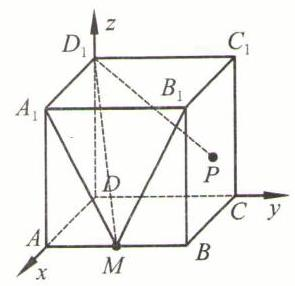
\includegraphics[width=0.2\textwidth]{bodyxb/src/bo_d20cdrf7aajc73bfmvhg_186_1182_435_295_286_0.jpg}
\end{center}


(第 66 题)

设 $P\left( {x,1,z}\right) ,\left( {x,z \in  \left( {0,1}\right) }\right)$ ,则 $\vv{M{B}_{1}} = \left( {0,\dfrac{1}{2},1}\right) ,\vv{{D}_{1}P} = \left( {x,1,z - 1}\right)$ .

若 $P{D}_{1} \bot  M{B}_{1}$ ,则 $\vv{M{B}_{1}} \cdot  \vv{{D}_{1}P} = \dfrac{1}{2} + z - 1 = 0$ ,解得 $z = \dfrac{1}{2}$ ,

所以存在点 $P$ 满足 $P{D}_{1} \bot  M{B}_{1}$ ,故①正确.

因为 $\vv{{D}_{1}{A}_{1}} = \left( {1,0,0}\right) ,\vv{{D}_{1}M} = \left( {1,\dfrac{1}{2}, - 1}\right)$ ,

设平面 ${A}_{1}{D}_{1}M$ 的法向量为 $\mathbf{n} = \left( {a,b,c}\right)$ ,则

$\left\{  \begin{array}{l} \mathbf{n} \cdot  \vv{{D}_{1}{A}_{1}} = a = 0, \\  \mathbf{n} \cdot  \vv{{D}_{1}M} = a + \dfrac{1}{2}b - c = 0, \end{array}\right.$ 取 $\mathbf{n} = \left( {0,2,1}\right) .$

设 $P{D}_{1}$ 与平面 ${A}_{1}{D}_{1}M$ 所成角为 $\theta$ ,

则 $\sin \theta  = \dfrac{\left| \vv{{D}_{1}P} \cdot  n\right| }{\left| \vv{{D}_{1}P}\right|  \cdot  \left| n\right| } = \dfrac{\left| z + 1\right| }{\sqrt{5} \times  \sqrt{{x}^{2} + 1 + {\left( z - 1\right) }^{2}}}$ ,

令 $x = 0,z = 1$ ,则 $\sin \theta  = \dfrac{2}{\sqrt{5}} = \dfrac{2\sqrt{5}}{5} > \dfrac{\sqrt{3}}{2}$ ,所以 $\theta  > {60}^{ \circ  }$ ,

令 $x = 0,z = 0$ ,则 $\sin \theta  = \dfrac{1}{\sqrt{10}} = \dfrac{\sqrt{10}}{10} < \dfrac{\sqrt{3}}{2}$ ,所以 $\theta  < {60}^{ \circ  }$ ,

所以存在点 $P$ 满足 $P{D}_{1}$ 与平面 ${A}_{1}{D}_{1}M$ 所成角的大小为 ${60}^{ \circ  }$ ,故②正确.

因为 $\left| \vv{{D}_{1}M}\right|  = \sqrt{{1}^{2} + {\left( \dfrac{1}{2}\right) }^{2} + {\left( -1\right) }^{2}} = \dfrac{3}{2},\vv{MP} = \left( {x - 1,\dfrac{1}{2},z}\right)$ ,

所以 $\left| \vv{MP}\right|  = \sqrt{{\left( x - 1\right) }^{2} + {z}^{2} + \dfrac{1}{4}} \in  \left( {\dfrac{1}{2},\dfrac{3}{2}}\right)$ ,所以 $M{D}_{1} + {MP} \in  \left( {2,3}\right)$ , 所以存在点 $P$ 满足 $M{D}_{1} + {MP} = \dfrac{12}{5}$ ,故③正确.

67. $\left\lbrack  {\dfrac{11}{5},5}\right\rbrack$ 提示: 如图,建立空间直角坐标系.

\begin{center}
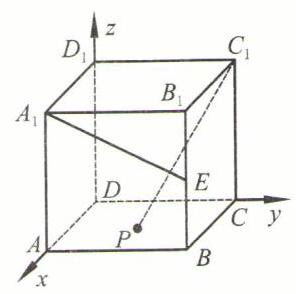
\includegraphics[width=0.2\textwidth]{bodyxb/src/bo_d20cdrf7aajc73bfmvhg_186_1191_1463_296_294_0.jpg}
\end{center}


(第 67 题)

因为 ${AB} = 2$ ,则 ${A}_{1}\left( {2,0,2}\right) ,{C}_{1}\left( {0,2,2}\right) ,{D}_{1}\left( {0,0,2}\right) ,E\left( {2,2,1}\right)$ .

设 $P\left( {x,y,z}\right) ,x,y,z \in  \left\lbrack  {0,2}\right\rbrack$ ,

因为 $\vv{{C}_{1}P} = \left( {x,y - 2,z - 2}\right) ,\vv{{A}_{1}E} = \left( {0,2, - 1}\right) ,{C}_{1}P \bot  {A}_{1}E$ ,所以 $2\left( {y - 2}\right)  - \left( {z - 2}\right)  = 0$ ,即 $z = {2y} - 2.$

由 $z = {2y} - 2 \in  \left\lbrack  {0,2}\right\rbrack$ ,得 $y \in  \left\lbrack  {1,2}\right\rbrack$ ,则 $P\left( {x,y,{2y} - 2}\right) ,x \in  \left\lbrack  {0,2}\right\rbrack  ,y \in  \left\lbrack  {1,2}\right\rbrack$ ,

则 $\vv{P{A}_{1}} = \left( {2 - x, - y,4 - {2y}}\right) ,\vv{P{D}_{1}} = \left( {-x, - y,4 - {2y}}\right)$ ,

则 $\vv{P{A}_{1}} \cdot  \vv{P{D}_{1}} = \left( {2 - x, - y,4 - {2y}}\right)  \cdot  \left( {-x, - y,4 - {2y}}\right)  = x\left( {x - 2}\right)  + {y}^{2} + {\left( 2y - 4\right) }^{2}$

$= {x}^{2} - {2x} + {y}^{2} + 4{y}^{2} - {16y} + {16} = {\left( x - 1\right) }^{2} + 5{\left( y - \dfrac{8}{5}\right) }^{2} + \dfrac{11}{5},$

所以当 $x = 1,y = \dfrac{8}{5}$ 时, $\vv{P{A}_{1}} \cdot  \vv{P{D}_{1}}$ 取得最小值 $\dfrac{11}{5}$ ;

当 $x = 0$ 或 $x = 2,y = 1$ 时, $\vv{P{A}_{1}} \cdot  \vv{P{D}_{1}}$ 取得最大值 5,

所以 $\vv{P{A}_{1}} \cdot  \vv{P{D}_{1}}$ 的取值范围是 $\left\lbrack  {\dfrac{11}{5},5}\right\rbrack$ .

68. 7 提示: 由题意知 $\vv{{B}_{1}{A}_{1}} = \left( {0,3,0}\right) ,\vv{{B}_{1}{C}_{1}} = \left( {4,0,0}\right) ,\vv{BA} = \left( {0,\dfrac{3}{2},0}\right) ,\vv{BC} = \left( {2,0,0}\right)$ ,

$\vv{{A}_{1}{C}_{1}} = \left( {4, - 3,0}\right) ,\vv{AC} = \left( {2, - \dfrac{3}{2},0}\right) ,\vv{{A}_{1}A} = \left( {0,0,2}\right)$ ,

所以 $\vv{{B}_{1}{A}_{1}} \cdot  \vv{{B}_{1}{C}_{1}} = 0,\vv{BA} \cdot  \vv{BC} = 0$ ,即 $\vv{{B}_{1}{A}_{1}} \bot  \vv{{B}_{1}{C}_{1}},\vv{BA} \bot  \vv{BC}$ .

又 $\vv{{B}_{1}{A}_{1}} = 2\vv{BA} = 0,\vv{{B}_{1}{C}_{1}} = 2\vv{BC},\vv{{A}_{1}{C}_{1}} = 2\vv{AC},\vv{{B}_{1}{A}_{1}} \cdot  \vv{{A}_{1}A} = 0,\vv{{B}_{1}{C}_{1}} \cdot  \vv{{A}_{1}A} = 0$ ,即 $\vv{{B}_{1}{A}_{1}}\bot \vv{{A}_{1}A},\vv{{B}_{1}{C}_{1}}\bot \vv{{A}_{1}A}$ ,

${B}_{1}{A}_{1} \cap  {B}_{1}{C}_{1} = {B}_{1},{B}_{1}{A}_{1},{B}_{1}{C}_{1} \subset$ 平面 ${A}_{1}{B}_{1}{C}_{1}$ ,所以 ${A}_{1}A \bot$ 平面 ${A}_{1}{B}_{1}{C}_{1}$ ,

所以这 6 个点是一个三棱台的 6 个顶点,且 $A{A}_{1}$ 与该三棱台的底面垂直.

又 ${A}_{1}{B}_{1} = 3,{B}_{1}{C}_{1} = 4,{AB} = \dfrac{3}{2},{BC} = 2,A{A}_{1} = 2$ ,所以几何体 ${ABC} - {A}_{1}{B}_{1}{C}_{1}$ 的体积:

\begin{center}
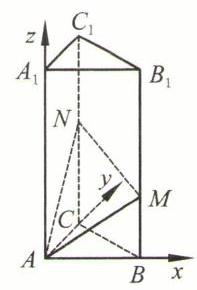
\includegraphics[width=0.2\textwidth]{bodyxb/src/bo_d20cdrf7aajc73bfmvhg_187_1248_381_197_290_0.jpg}
\end{center}


(第 69 题)

${V}_{{ABC} - {A}_{1}{B}_{1}{C}_{1}} = \dfrac{1}{3} \times  2 \times  \left( {\dfrac{1}{2} \times  3 \times  4 + \dfrac{1}{2} \times  \dfrac{3}{2} \times  2 + \sqrt{\dfrac{1}{2} \times  3 \times  4 \times  \dfrac{1}{2} \times  \dfrac{3}{2} \times  2}}\right)  = 7.$

69. $\dfrac{\pi }{3}$ 提示:如图,建立空间直角坐标系. 依题意,设 ${BM} = a,{CN} = b,{AB} = 1$ ,则 $A{A}_{1} = 2,{AB} = 1$ ,

则 $A\left( {0,0,0}\right) ,B\left( {1,0,0}\right) ,M\left( {1,0,a}\right) ,N\left( {0,1,b}\right) ,\vv{AM} = \left( {1,0,a}\right) ,\vv{AN} = \left( {0,1,b}\right)$ .

设平面 ${AMN}$ 的法向量为 $\mathbf{m} = \left( {x,y,z}\right)$ ,则 $\left\{  \begin{array}{l} \vv{AM} \cdot  \mathbf{m} = x + {az} = 0, \\  \vv{AN} \cdot  \mathbf{m} = y + {bz} = 0, \end{array}\right.$

令 $z =  - 1$ ,得 $\mathbf{m} = \left( {a,b, - 1}\right)$ .

平面 ${ABC}$ 的法向量 $\mathbf{n} = \left( {0,0,1}\right)$ ,

由平面 ${AMN}$ 与平面 ${ABC}$ 所成 (锐) 二面角为 $\dfrac{\pi }{6}$ ,得 $\cos \dfrac{\pi }{6} = \dfrac{\left| m \cdot  n\right| }{\left| m\right| \left| n\right| } = \dfrac{1}{\sqrt{{a}^{2} + {b}^{2} + 1}}$ ,

化简得 ${a}^{2} + {b}^{2} = \dfrac{1}{3}$ ,当 $a$ 取得最大值时, ${B}_{1}M$ 最小,此时 $b = 0,{a}_{\max } = \dfrac{\sqrt{3}}{3}$ ,

且 $\tan \angle {AMB} = \dfrac{AB}{MB} = \sqrt{3}$ ,所以 $\angle {AMB} = \dfrac{\pi }{3}$ .

70. $\dfrac{\sqrt{21}}{7}$ 提示: 取 ${BD},{AC}$ 交点于点 $O$ . 因为直四棱柱 ${ABCD} - {A}_{1}{B}_{1}{C}_{1}{D}_{1}$ 的所有棱长都为 2, $\angle {BAD} = \dfrac{\pi }{3}$ ,所以 ${BD}\bot {AC}$ ,建立如图所示空间直角坐标系.

\begin{center}
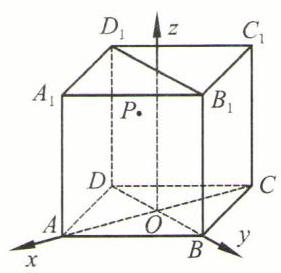
\includegraphics[width=0.2\textwidth]{bodyxb/src/bo_d20cdrf7aajc73bfmvhg_187_1166_1030_281_273_0.jpg}
\end{center}


(第 70 题)

所以 $A\left( {\sqrt{3},0,0}\right) ,C\left( {-\sqrt{3},0,0}\right) ,{D}_{1}\left( {0, - 1,2}\right) ,{B}_{1}\left( {0,1,2}\right) ,\vv{A{D}_{1}} = \left( {-\sqrt{3}, - 1,2}\right)$ ,

$\vv{A{B}_{1}} = \left( {-\sqrt{3},1,2}\right)$ . 设平面 $A{D}_{1}{B}_{1}$ 的法向量为 $\mathbf{n} = \left( {x,y,z}\right)$ ,

则有 $\left\{  \begin{array}{l} \mathbf{n} \cdot  \vv{A{D}_{1}} =  - \sqrt{3}x - y + {2z} = 0, \\  \mathbf{n} \cdot  \vv{A{B}_{1}} =  - \sqrt{3}x + y + {2z} = 0, \end{array}\right.$

令 $x = 2$ ,则 $y = 0,z = \sqrt{3}$ ,所以 $\mathbf{n} = \left( {2,0,\sqrt{3}}\right)$ .

因为点 $P$ 在四边形 ${BD}{D}_{1}{B}_{1}$ 及其内部运动,所以设 $P\left( {0,y,z}\right) ,\left( {-1 \leq  y \leq  1,0 \leq  z \leq  2}\right)$ .

又因为 $\left| {PA}\right|  + \left| {PC}\right|  = 4$ ,所以 $\sqrt{{\left( -\sqrt{3}\right) }^{2} + {y}^{2} + {z}^{2}} + \sqrt{{\left( \sqrt{3}\right) }^{2} + {y}^{2} + {z}^{2}} = 4$ ,即 ${y}^{2} + {z}^{2} = 1$ ,则 $- 1 \leq  y \leq  1,0 \leq  z \leq  1$ .

设点 $P$ 到平面 $A{D}_{1}{B}_{1}$ 的距离为 $d$ ,则有 $d = \dfrac{\left| \vv{AP} \cdot  \mathbf{n}\right| }{\left| \mathbf{n}\right| } = \dfrac{\left| -\sqrt{3} \times  2 + \sqrt{3}z\right| }{\sqrt{{2}^{2} + {\left( \sqrt{3}\right) }^{2}}} = \dfrac{\left| \sqrt{3}z - 2\sqrt{3}\right| }{\sqrt{7}}$ .

又因为 $0 \leq  z \leq  1$ ,所以 $z = 1$ 时, ${d}_{\min } = \dfrac{\left| \sqrt{3} - 2\sqrt{3}\right| }{\sqrt{7}} = \dfrac{\sqrt{21}}{7}$ ,

即点 $P$ 到平面 $A{D}_{1}{B}_{1}$ 的距离的最小值为 $\dfrac{\sqrt{21}}{7}$ .

71. ②③④ 提示:由题意可将图形补全为一个正方体 ${ABEM} - {DCFN}$ ,如图建立空间直角坐标系.

\begin{center}
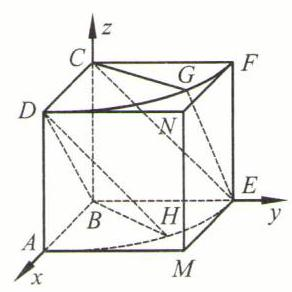
\includegraphics[width=0.2\textwidth]{bodyxb/src/bo_d20cdrf7aajc73bfmvhg_187_1155_1754_292_292_0.jpg}
\end{center}


(第 71 题)

则 $B\left( {0,0,0}\right) ,C\left( {0,0,2}\right) ,D\left( {2,0,2}\right) ,A\left( {2,0,0}\right) ,F\left( {0,2,2}\right) ,E\left( {0,2,0}\right) ,G\left( {\sqrt{2},\sqrt{2},2}\right)$ .

设点 $H\left( {2\cos \alpha ,2\sin \alpha ,0}\right)$ ,其中 $0 \leq  \alpha  \leq  \dfrac{\pi }{2}$ ,

对于①, $\vv{CE} = \left( {0,2, - 2}\right) ,\vv{CG} = \left( {\sqrt{2},\sqrt{2},0}\right)$ ,设 $n = \left( {x,y,z}\right)$ 为平面 ${CEG}$ 的法向量,

则 $\left\{  \begin{array}{l} \mathbf{n} \cdot  \vv{CE} = 0, \\  \mathbf{n} \cdot  \vv{CG} = 0, \end{array}\right.$ 即 $\left\{  \begin{array}{l} {2y} - {2z} = 0, \\  \sqrt{2}x + \sqrt{2}y = 0, \end{array}\right.$ 取 $x = 1$ ,则 $y =  - 1,z =  - 1$ ,可得 $\mathbf{n} = \left( {1, - 1, - 1}\right)$ .

设 $\mathbf{m} = \left( {{x}_{1},{y}_{1},{z}_{1}}\right)$ 为平面 ${BDH}$ 的法向量, $\vv{BD} = \left( {2,0,2}\right) ,\vv{BH} = \left( {2\cos \alpha ,2\sin \alpha ,0}\right)$ ,

则 $\left\{  \begin{array}{l} \mathbf{m} \cdot  \vv{BD} = 0, \\  \mathbf{m} \cdot  \vv{BH} = 0, \end{array}\right.$ 即 $\left\{  \begin{array}{l} {2x} + {2z} = 0, \\  2\cos {\alpha x} + 2\sin {\alpha y} = 0, \end{array}\right.$ 同理可得 $\mathbf{m} = \left( {\sin \alpha , - \cos \alpha , - \sin \alpha }\right)$ .

若平面 ${BDH}//$ 平面 ${CEG}$ ,则 $\dfrac{\sin \alpha }{1} = \dfrac{-\cos \alpha }{-1} = \dfrac{-\sin \alpha }{-1}$ ,解得 $\alpha  = \dfrac{\pi }{4}$ ,

所以存在 $H\left( {\sqrt{2},\sqrt{2},0}\right)$ ,使得平面 ${BDH}//$ 平面 ${CEG}$ ,故①错误.

对于②, $\vv{FH} = \left( {2\cos \alpha ,2\sin \alpha  - 2, - 2}\right)$ ,若 ${FH} \bot$ 平面 ${CEG}$ ,

则 $\vv{FH}//\mathbf{n}$ ,即 $\dfrac{2\cos \alpha }{1} = \dfrac{2\sin \alpha  - 2}{-1} = \dfrac{-2}{-1}$ ,

解得 $\cos \alpha  = 1,\sin \alpha  = 0$ ,故存在点 $H\left( {2,0,0}\right)$ ,使得 ${FH} \bot$ 平面 ${CEG}$ ,故②正确.

对于③, $\vv{CH} = \left( {2\cos \alpha ,2\sin \alpha , - 2}\right)$ ,点 $H$ 到平面 ${CEG}$ 的距离为 $d$ ,

$d = \dfrac{\left| \vv{CH} \cdot  \mathbf{n}\right| }{\left| \mathbf{n}\right| } = \dfrac{\left| 2\cos \alpha  - 2\sin \alpha  + 2\right| }{\sqrt{3}} = \dfrac{\left| 2\sqrt{2}\sin \left( \alpha  + \dfrac{3\pi }{4}\right)  + 2\right| }{\sqrt{3}}.$

因为 $0 \leq  \alpha  \leq  \dfrac{\pi }{2}$ ,所以 $\dfrac{3\pi }{4} \leq  \alpha  + \dfrac{3\pi }{4} \leq  \dfrac{5\pi }{4}$ ,所以 $\sin \left( {\alpha  + \dfrac{3\pi }{4}}\right)  \in  \left\lbrack  {-\dfrac{\sqrt{2}}{2},\dfrac{\sqrt{2}}{2}}\right\rbrack$ ,

$2\sqrt{2}\sin \left( {\alpha  + \dfrac{3\pi }{4}}\right)  + 2 \in  \left\lbrack  {0,4}\right\rbrack$ ,所以 $d = \dfrac{\left| 2\sqrt{2}\sin \left( \alpha  + \dfrac{3\pi }{4}\right)  + 2\right| }{\sqrt{3}} \in  \left\lbrack  {0,\dfrac{4\sqrt{3}}{3}}\right\rbrack$ ,

所以不存在点 $H$ ,使得点 $H$ 到平面 ${CEG}$ 的距离大于 $\dfrac{4\sqrt{3}}{3}$ ,故③正确.

对于④, $\vv{DH} = \left( {2\cos \alpha  - 2,2\sin \alpha , - 2}\right) ,n = \left( {1, - 1, - 1}\right)$ ,直线 ${DH}$ 与平面 ${CEG}$ 的所成角 $\theta$ ,满足 $\sin \theta  = \dfrac{\left| \vv{DH} \cdot  n\right| }{\left| \vv{DH}\right|  \cdot  \left| n\right| } =$

$\dfrac{\left| 2\cos \alpha  - 2 - 2\sin \alpha  + 2\right| }{\sqrt{{\left( 2\cos \alpha  - 2\right) }^{2} + 4{\sin }^{2}\alpha  + 4} \cdot  \sqrt{3}} = \dfrac{\left| \cos \alpha  - \sin \alpha \right| }{\sqrt{3} \cdot  \sqrt{3 - 2\cos \alpha }} = \dfrac{\sqrt{2}}{3},$

整理可得 $3\sin {2\alpha } - 4\cos \alpha  + 3 = 0$ ,记 $f\left( \alpha \right)  = 3\sin {2\alpha } - 4\cos \alpha  + 3$ .

因为函数 $y = f\left( \alpha \right)$ 在 $\alpha  \in  \left\lbrack  {0,\dfrac{\pi }{2}}\right\rbrack$ 时的图像是连续的,且 $f\left( 0\right)  =  - 1 < 0,f\left( \dfrac{\pi }{2}\right)  = 3 > 0$ , 所以,存在 ${\alpha }_{0} \in  \left( {0,\dfrac{\pi }{2}}\right)$ ,使得 $f\left( {\alpha }_{0}\right)  = 0$ .

所以,存在点 $H$ ,使得直线 ${DH}$ 与平面 ${CEG}$ 的所成角的余弦值为 $\dfrac{\sqrt{2}}{3}$ ,④正确.

\begin{center}
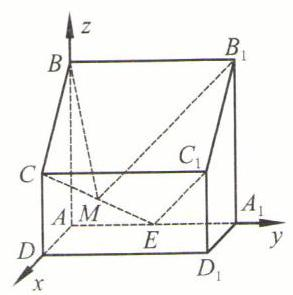
\includegraphics[width=0.2\textwidth]{bodyxb/src/bo_d20cdrf7aajc73bfmvhg_188_1191_1246_293_295_0.jpg}
\end{center}


(第 72 题)

72. (1) 由 $A{A}_{1} \bot$ 底面 ${ABCD},{AD},{AB} \subset$ 平面 ${ABCD}$ ,得 $A{A}_{1} \bot  {AD},A{A}_{1} \bot  {AB}$ ,而 ${AB} \bot  {AD}$ , 即直线 ${AD},A{A}_{1},{AB}$ 两两垂直.

如图,以 $A$ 为坐标原点,分别以 $\vv{AD},\vv{A{A}_{1}}$ 与 $\vv{AB}$ 为 $x,y$ 与 $z$ 轴的正方向,建立空间直角坐标系. 则

$B\left( {0,0,2}\right) ,D\left( {1,0,0}\right) ,C\left( {1,0,1}\right) ,{C}_{1}\left( {1,2,1}\right) ,{B}_{1}\left( {0,2,2}\right) ,E\left( {0,1,0}\right) ,M\left( {\dfrac{1}{2},\dfrac{1}{2},\dfrac{1}{2}}\right)$ , $\vv{E{C}_{1}} = \left( {1,1,1}\right) ,\vv{BC} = \left( {1,0, - 1}\right)$ ,显然 $\vv{BC} \cdot  \vv{E{C}_{1}} = 1 \times  1 - 1 \times  1 = 0$ ,即 $\vv{BC} \bot  \vv{E{C}_{1}}$ ,所以 ${BC} \bot  {C}_{1}E$ .

(2) $\vv{BM} = \left( {\dfrac{1}{2},\dfrac{1}{2}, - \dfrac{3}{2}}\right) ,\vv{AD} = \left( {1,0,0}\right) ,\cos \langle \vv{BM},\vv{AD}\rangle  = \dfrac{\vv{BM} \cdot  \vv{AD}}{\left| \vv{BM}\right| \left| \vv{AD}\right| } = \dfrac{\dfrac{1}{2}}{\sqrt{{\left( \dfrac{1}{2}\right) }^{2} + {\left( \dfrac{1}{2}\right) }^{2} + {\left( -\dfrac{3}{2}\right) }^{2}}} = \dfrac{\sqrt{11}}{11}$ ,

所以异面直线 ${BM}$ 与 ${AD}$ 所成角的余弦值为 $\dfrac{\sqrt{11}}{11}$ .

(3) $\vv{BM} = \left( {\dfrac{1}{2},\dfrac{1}{2}, - \dfrac{3}{2}}\right) ,\vv{B{B}_{1}} = \left( {0,2,0}\right) ,\vv{{C}_{1}{B}_{1}} = \left( {-1,0,1}\right)$ .

设平面 ${BM}{B}_{1}$ 的法向量 $\mathbf{n} = \left( {x,y,z}\right)$ ,则 $\left\{  \begin{array}{l} \mathbf{n} \cdot  \vv{B{B}_{1}} = {2y} = 0, \\  \mathbf{n} \cdot  \vv{BM} = \dfrac{1}{2}x + \dfrac{1}{2}y - \dfrac{3}{2}z = 0, \end{array}\right.$ 令 $z = 1$ ,得 $\mathbf{n} = \left( {3,0,1}\right)$ ,

所以点 ${C}_{1}$ 到平面 ${BM}{B}_{1}$ 的距离 $d = \dfrac{\left| \mathbf{n} \cdot  \vv{{C}_{1}{B}_{1}}\right| }{\left| \mathbf{n}\right| } = \dfrac{2}{\sqrt{10}} = \dfrac{\sqrt{10}}{5}$ .

73. (1) 在棱 ${BC}$ 上存在点 $N$ ,使得 ${CM}//$ 平面 ${PAN}$ ,点 $N$ 为棱 ${BC}$ 的中点.

证明如下: 取 ${PA}$ 的中点 $Q$ ,连接 ${NQ},{MQ}$ .

\begin{center}
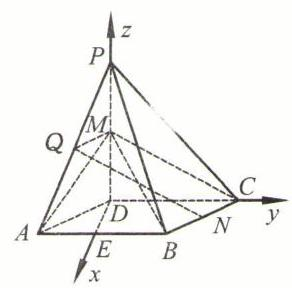
\includegraphics[width=0.2\textwidth]{bodyxb/src/bo_d20cdrf7aajc73bfmvhg_189_1147_145_292_288_0.jpg}
\end{center}


(第 73 题)

由题意, ${MQ}//{AD}$ 且 ${MQ} = \dfrac{1}{2}{AD},{CN}//{AD}$ 且 ${CN} = \dfrac{1}{2}{AD}$ ,

故 ${CN}//{MQ}$ 且 ${CN} = {MQ}$ . $\therefore$ 四边形 ${CNQM}$ 为平行四边形.

$\therefore {CM}//{NQ}$ ,又 ${CM} ⊄$ 平面 ${PAN},{NQ} \subset$ 平面 ${PAN},\therefore {CM}//$ 平面 ${PAN}$ .

(2)取 ${AB}$ 中点 $E$ ,因为底面 ${ABCD}$ 为菱形,所以 ${AC} \bot  {BD}$ .

又 ${PB} \bot  {AC}$ ,且 ${PB} \cap  {BD} = B$ ,所以 ${AC} \bot$ 平面 ${PBD}$ ,即 ${PD} \bot  {AC}$ .

又 $\angle {PDC} = \dfrac{\pi }{2}$ ,即 ${PD} \bot  {DC}$ ,而 ${DC} \cap  {AC} = C$ ,所以 ${PD} \bot$ 平面 ${ABCD}$ .

又 $\angle {ABC} = 2\angle {BAD}$ ,所以 $\bigtriangleup {ABD}$ 为正三角形,即 ${DE}\bot {AB}$ ,也即 ${DE}\bot {DC}$

所以 ${DE},{DC},{DP}$ 两两互相垂直.

以 $D$ 为坐标原点,分别以 $\vv{DE},\vv{DC}$ 与 $\vv{DP}$ 为 $x,y$ 与 $z$ 轴的正方向,建立空间直角坐标系. 设 ${MD} = a$ ,则 $M\left( {0,0,a}\right)$ ,

$C\left( {0,2,0}\right) ,B\left( {\sqrt{3},1,0}\right) ,A\left( {\sqrt{3}, - 1,0}\right)$ .

所以 $\vv{MC} = \left( {0,2, - a}\right) ,\vv{CB} = \left( {\sqrt{3}, - 1,0}\right)$ .

设平面 ${MBC}$ 的一个法向量为 $m = \left( {x,y,z}\right)$ . 由 $\left\{  \begin{array}{l} m \cdot  \vv{MC} = {2y} - {az} = 0, \\  m \cdot  \vv{CB} = \sqrt{3}x - y = 0, \end{array}\right.$ 取 $x = 1$ ,得 $m = \left( {1,\sqrt{3},\dfrac{2\sqrt{3}}{a}}\right)$ .

取平面 ${DMC}$ 的一个法向量为 $\mathbf{n} = \left( {1,0,0}\right)$ .

由题意, $\dfrac{\sqrt{6}}{6} = \left| {\cos \langle \mathbf{m},\mathbf{n}\rangle }\right|  = \dfrac{1}{\sqrt{1 + 3 + \dfrac{12}{{a}^{2}}}}$ ,解得 $a = \sqrt{6}$ .

又 $\vv{MA} = \left( {\sqrt{3}, - 1, - \sqrt{6}}\right)$ ,则点 $A$ 到平面 ${BCM}$ 的距离 $d = \dfrac{\left| m \cdot  \vv{MA}\right| }{\left| m\right| } = \dfrac{2\sqrt{3}}{\sqrt{6}} = \sqrt{2}$ .

74. (1) 在图 1 中,过 $B$ 作 ${BF}\bot {CD}$ ,所以 ${CF} = 1$ ,又 $\angle {DCB} = {60}^{ \circ  }$ ,所以 ${BC} = 2$ ,所以 $\bigtriangleup  {BCE}$ 是等边三角形; 连接 ${AE}$ ,可得: $\bigtriangleup {ABE}$ 也是等边三角形.

\begin{center}
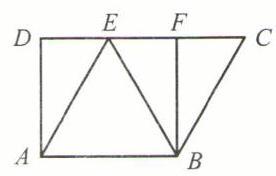
\includegraphics[width=0.2\textwidth]{bodyxb/src/bo_d20cdrf7aajc73bfmvhg_189_1163_1017_276_176_0.jpg}
\end{center}


(图 1)

在图 2 中取 ${BE}$ 中点 $O$ ,连接 ${C}_{1}O,{AO}$ .

因为 ${C}_{1}O = {AO} = \sqrt{3},A{C}_{1} = \sqrt{6}$ ,所以 ${C}_{1}{O}^{2} + A{O}^{2} = A{C}_{1}^{2}$ ,所以 ${C}_{1}O \bot  {AO}$ . 且 ${C}_{1}O \bot  {OB}$ ,

${OA} \cap  {OB} = O,{OA} \subset$ 平面 ${ABED},{OB} \subset$ 平面 ${ABED}$ ,所以 ${C}_{1}O \bot$ 平面 ${ABED}$ , ${C}_{1}O \subset$ 平面 $B{C}_{1}E$ ,所以平面 $B{C}_{1}E \bot$ 平面 ${ABED}$ .

(2)因为 ${C}_{1}O,{OB},{OA}$ 两两垂直,可以以 $O$ 为原点,建立如图 3 所示的空间直角坐标系.

\begin{center}
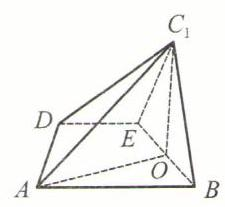
\includegraphics[width=0.2\textwidth]{bodyxb/src/bo_d20cdrf7aajc73bfmvhg_189_1217_1259_225_207_0.jpg}
\end{center}


(图 2)

则 $D\left( {\dfrac{\sqrt{3}}{2}, - \dfrac{3}{2},0}\right) ,{C}_{1}\left( {0,0,\sqrt{3}}\right) ,E\left( {0, - 1,0}\right) ,B\left( {0,1,0}\right)$ ,

$\vv{D{C}_{1}} = \left( {-\dfrac{\sqrt{3}}{2},\dfrac{3}{2},\sqrt{3}}\right) ,\vv{BE} = \left( {0, - 2,0}\right) ,\vv{BD} = \left( {\dfrac{\sqrt{3}}{2}, - \dfrac{5}{2},0}\right) .$

设 $\vv{DP} = \lambda \vv{D{C}_{1}} = \left( {-\dfrac{\sqrt{3}}{2}\lambda ,\dfrac{3}{2}\lambda ,\sqrt{3}\lambda }\right) ,0 \leq  \lambda  \leq  1$ ,

所以 $\vv{BP} = \vv{BD} + \vv{DP} = \left( {\dfrac{\sqrt{3}}{2} - \dfrac{\sqrt{3}}{2}\lambda , - \dfrac{5}{2} + \dfrac{3}{2}\lambda ,\sqrt{3}\lambda }\right)$ .

\begin{center}
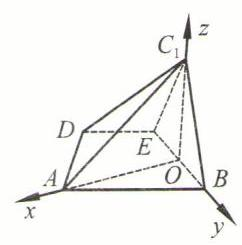
\includegraphics[width=0.2\textwidth]{bodyxb/src/bo_d20cdrf7aajc73bfmvhg_189_1200_1533_242_245_0.jpg}
\end{center}


(图 3)

(第 74 题)

取平面 ${ABE}$ 的法向量 $\mathbf{n} = \left( {0,0,1}\right)$ . 设平面 ${PBE}$ 的法向量 $\mathbf{m} = \left( {x,y,z}\right)$ ,

则 $\left\{  \begin{array}{l} \mathbf{m} \cdot  \vv{BE} =  - {2y} = 0, \\  \mathbf{m} \cdot  \vv{BP} = \left( {\dfrac{\sqrt{3}}{2} - \dfrac{\sqrt{3}}{2}\lambda }\right) x + \left( {-\dfrac{5}{2} + \dfrac{3}{2}\lambda }\right) y + \sqrt{3}{\lambda z} = 0, \end{array}\right.$ 可取 $\mathbf{m} = \left( {{2\lambda },0,\lambda  - 1}\right)$ .

因为锐二面角 $P - {BE} - A$ 的大小为 ${45}^{ \circ  }$ ,

所以 $\left| {\cos \langle \mathbf{m},\mathbf{n}\rangle }\right|  = \dfrac{\left| \lambda  - 1\right| }{\sqrt{4{\lambda }^{2} + {\left( \lambda  - 1\right) }^{2}}} = \dfrac{\sqrt{2}}{2}$ ,解得 $\lambda  = \dfrac{1}{3}\left( {\lambda  =  - 1\text{ 舍 }}\right)$ .

所以平面 ${PBE}$ 的法向量 $\mathbf{m} = \left( {\dfrac{2}{3},0, - \dfrac{2}{3}}\right) ,\vv{B{C}_{1}} = \left( {0, - 1,\sqrt{3}}\right)$ .

所以点 ${C}_{1}$ 到平面 ${PBE}$ 的距离 $d = \dfrac{\left| \vv{B{C}_{1}} \cdot  m\right| }{\left| m\right| } = \dfrac{\sqrt{6}}{2}$ .

75. 以 $D$ 为坐标原点,分别以 $\vv{DA},\vv{DC},\vv{D{D}_{2}}$ 的方向为 $x,y$ 与 $z$ 轴的正方向,建立空间直角坐标系,则 ${A}_{1}\left( {4,0,1}\right) \text{ 、 }{C}_{1}(0,4$ ,

1). 设 $P\left( {x,y,4}\right)$ ,其中 ${x}^{2} + {y}^{2} = 2\left( {0 \leq  x \leq  \sqrt{2},0 \leq  y \leq  \sqrt{2}}\right) .\vv{{A}_{1}{C}_{1}} = \left( {-4,4,0}\right) ,\vv{{A}_{1}P} = \left( {x - 4,y,3}\right)$ .

设平面 $P{A}_{1}{C}_{1}$ 的法向量为 $\mathbf{n} = \left( {u,v,w}\right)$ ,则 $\left\{  \begin{array}{l} \mathbf{n} \cdot  \vv{{A}_{1}{C}_{1}} =  - {4u} + {4v} = 0, \\  \mathbf{n} \cdot  \vv{{A}_{1}P} = \left( {x - 4}\right) u + {yv} + {3w} = 0, \end{array}\right.$

\begin{center}
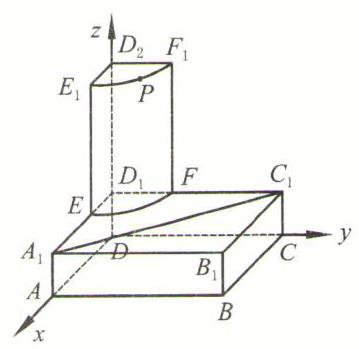
\includegraphics[width=0.3\textwidth]{bodyxb/src/bo_d20cdrf7aajc73bfmvhg_190_1116_114_359_349_0.jpg}
\end{center}


(第 75 题)

取 $u = 1$ ,从而得平面 $P{A}_{1}{C}_{1}$ 的一个法向量为 $\mathbf{n} = \left( {1,1,\dfrac{4 - \left( {x + y}\right) }{3}}\right)$ .

平面 ${ABC}$ 的一个法向量可取为 $\mathbf{m} = \left( {0,0,1}\right)$ .

设平面 $P{A}_{1}{C}_{1}$ 与平面 ${ABC}$ 所成的钝二面角的平面角的大小为 $\theta$ .

于是 $\cos \theta  =  - \left| {\cos \langle \mathbf{m},\mathbf{n}\rangle }\right|  =  - \dfrac{\left| \dfrac{4 - \left( {x + y}\right) }{3}\right| }{1 \times  \sqrt{1 + 1 + {\left( \dfrac{4 - \left( {x + y}\right) }{3}\right) }^{2}}}$ .

设 $t = \dfrac{4 - \left( {x + y}\right) }{3} \in  \left\lbrack  {\dfrac{2}{3},\dfrac{4 - \sqrt{2}}{3}}\right\rbrack$ ,则 $\cos \theta  =  - \dfrac{t}{\sqrt{1 + 1 + {t}^{2}}} =  - \dfrac{1}{\sqrt{2{\left( \dfrac{1}{t}\right) }^{2} + 1}}$ .

因为平面 $P{A}_{1}{C}_{1}$ 与平面 ${ABC}$ 成的钝二面角最大时,其余弦值最小,且函数 $y =  - \dfrac{1}{\sqrt{2\left( \dfrac{1}{{t}^{2}}\right)  + 1}}$ 在区间 $\left\lbrack  {\dfrac{2}{3},\dfrac{4 - \sqrt{2}}{3}}\right\rbrack$ 上是

严格减函数,所以 $t = \dfrac{4 - \sqrt{2}}{3}$ 时,平面 $P{A}_{1}{C}_{1}$ 与平面 ${ABC}$ 所成的钝二面角最大,此时点 $P$ 即点 ${E}_{1}$ 或点 ${F}_{1}$ .

